%&../preamble

\def\npart {IB}
\def\nterm {Lent}
\def\nyear {2022}
\def\nlecturer {Prof. S. Bacallado}
\def\ncourse {Statistics}

\def\encodingdefault{TU}\normalfont
\ifnum 0\ifxetex 1\fi\ifluatex 1\fi=0 % if pdftex
  \usepackage[T1]{fontenc}
  \usepackage[utf8]{inputenc}
  \usepackage{textcomp} % provide euro and other symbols
\else % if luatex or xetex
  % \usepackage{unicode-math}
  % \defaultfontfeatures{Scale=MatchLowercase}
  % \defaultfontfeatures[\rmfamily]{Ligatures=TeX,Scale=1}
  % \DeclareMathAlphabet{\mathcal}{OMS}{cmsy}{m}{n}
  % \let\mathbb\relax % remove the definition by unicode-math
  % \DeclareMathAlphabet{\mathbb}{U}{msb}{m}{n}
\fi

\usetikzlibrary{external}
\tikzset{external/system call={xelatex -fmt=../preamble.fmt \tikzexternalcheckshellescape -halt-on-error -interaction=batchmode -jobname "\image" "\texsource"}} % path is relative to file that includes preamble
\tikzexternalize

\providetoggle{DontSetTitleAuthorDate}

\nottoggle{DontSetTitleAuthorDate}{
  \hypersetup{
    pdftitle={Part \npart\ - \ncourse},
    pdfsubject={Cambridge Maths Notes: Part \npart\ - \ncourse},
    pdfkeywords={Cambridge Mathematics Maths Math \npart\ \nterm\ \nyear\ \ncourse}
  }

  \author{Based on lectures by \nlecturer}
  \date{\nterm\ \nyear}
  \title{Part \npart\ --- \ncourse}
}{}

\tikzsetexternalprefix{figtemp/}
\author{Based on lectures by \nlecturer \ and notes by thirdsgames.co.uk}

\newcommand{\prob}[1]{\mathbb{P}\left({#1}\right)}
\newcommand{\psub}[2]{\mathbb{P}_{#1}\left({#2}\right)}
\newcommand{\psubx}[1]{\psub{x}{#1}}
\newcommand{\expect}[1]{\mathbb{E}\left[{#1}\right]}
\newcommand{\esub}[2]{\mathbb{E}_{#1}\left[{#2}\right]}
\newcommand{\esubx}[1]{\esub{x}{#1}}
\newcommand{\Corr}[1]{\Corr\left({#1}\right)}
\newcommand{\convdist}{\xrightarrow{d}}
\newcommand{\convprob}{\xrightarrow{\mathbb{P}}}
\DeclareMathOperator{\Varop}{Var}
\renewcommand{\Var}[1]{\Varop\left({#1}\right)}
\newcommand{\Varsub}[2]{\Varop_{#1}\left({#2}\right)}

\newcommand{\tran}{\intercal}
\newcommand{\wildcard}{{}\cdot{}}

\begin{document}
    \maketitle
    \tableofcontents

    \section{Introduction and review of IA Probability}

\subsection{Introduction}
Statistics can be defined as the science of making informed decisions.
The field comprises, for example:
\begin{itemize}
	\item the design of experiments and studies;
	\item visualisation of data;
	\item formal statistical inference (which is the focus of this course);
	\item communication of uncertainty and risk; and
	\item formal decision theory.
\end{itemize}
This course concerns itself with \textit{parametric inference}.
Let $X_1, \dots, X_n$ be i.i.d.\ (independent and identically distributed) random variables, where we assume that the distribution of $X_1$ belongs to some family with parameter $\theta \in \Theta$.
For instance, let $X_1 \sim \mathrm{Poisson}(\mu)$, where $\theta = \mu$ and $\Theta = (0, \infty)$.
Another example is $X_1 \sim N(\mu, \sigma^2)$, and $\theta = (\mu, \sigma^2)$ and $\Theta = \mathbb R \times (0, \infty)$.
We use the observed $X = (X_1, \dots, X_n)$ to make inferences about the parameter $\theta$:
\begin{enumerate}
	\item we can estimate the value of $\theta$ using a \textit{point estimate} written $\hat \theta(X)$;
	\item we can make an \textit{interval estimate} of $\theta$, written $(\hat \theta_1(X), \hat \theta_2(X))$;
	\item hypotheses about $\theta$ can be tested, for instance the hypothesis $H_0 \colon \theta = 1$, by checking whether there is evidence in the data $X$ against the hypothesis $H_0$.
\end{enumerate}
\begin{remark}
	In general, we will assume that the family of distributions of the observations $X_i$ is known \textit{a priori}, and the parameter $\theta$ is the only unknown.
	There will, however, be some remarks later in the course where we can make weaker assumptions about the family.
\end{remark}

\subsection{Review of IA Probability}
\textit{This subsection reviews material covered in the IA Probability course.
	Some keywords are measure-theoretic, and are not defined.}

Let $\Omega$ be the \textit{sample space} of outcomes in an experiment.
A \textit{measurable} subset of $\Omega$ is called an \textit{event}, and we denote the set of events by $\mathcal F$.
A \textit{probability measure} $\mathbb P \colon \mathcal F \to [0,1]$ satisfies the following properties.
\begin{enumerate}
	\item $\prob{\varnothing} = 0$;
	\item $\prob{\Omega} = 1$;
	\item $\prob{\bigcup_{i = 1}^\infty A_i} = \sum_{i=1}^\infty \prob{A_i}$ if $(A_i)$ is a sequence of disjoint events.
\end{enumerate}
A \textit{random variable} is a \textit{measurable function} $X \colon \Omega \to \mathbb R$.
The \textit{distribution function} of a random variable $X$ is the function $F_X(x) = \prob{X \leq x}$.
We say that a random variable is \textit{discrete} when it takes values in a countable set $\mathcal X \subset \mathbb R$.
The \textit{probability mass function} of a discrete random variable is the function $p_X(x) = \prob{X = x}$.
We say that $X$ has a \textit{continuous distribution} if it has a \textit{probability density function} $f_X(x)$ such that $\prob{x \in A} = \int_A f_X(x) \dd{x}$ for `nice' sets $A$.

The \textit{expectation} of a random variable $X$ is defined as
\begin{align*}
	\expect{X} = \begin{cases}
		\sum_{x \in X} x p_X(x)               & \text{if } X \text{ discrete}   \\
		\int_{-\infty}^\infty x f_X(x) \dd{x} & \text{if } X \text{ continuous}
	\end{cases}
\end{align*}
If $g \colon \mathbb R \to \mathbb R$, we define $\expect{g(X)}$ by considering the fact that $g(X)$ is also a random variable.
For instance, in the continuous case,
\begin{align*}
	\expect{g(X)} = \int_{-\infty}^\infty g(x) f_X(x) \dd{x}
\end{align*}
The \textit{variance} of a random variable $X$ is defined as $\expect{(X - \expect{X})^2}$.

We say that a set of random variables $X_1, \dots, X_n$ are \textit{independent} if, for all $x_1, \dots, x_n$, we have
\begin{align*}
	\prob{X_1 \leq x_1, \dots, X_n \leq x_n} = \prob{X_1 \leq x_1} \cdots \prob{X_n \leq x_n}
\end{align*}
If and only if $X_1, \dots, X_n$ have probability density (or mass) functions $f_1, \dots, f_n$, then the \textit{joint probability density (respectively mass) function} is
\begin{align*}
	f_X(x) = \prod_{i = 1}^n f_{X_i}(x_i)
\end{align*}

If $Y = \max\qty{X_1, \dots, X_n}$ where the $X_i$ are independent, then the distribution function of $Y$ is given by
\begin{align*}
	\prob{Y \leq y} = \prob{X_1 \leq y} \cdots \prob{X_n \leq y}
\end{align*}
The probability density function of $Y$ (if it exists) is obtained by the differentiating the above.

Under a linear transformation, the expectation and variance have certain properties.
Let $a = (a_1, \dots, a_n)^\tran \in \mathbb R^n$ be a constant in $\mathbb R^n$.
\begin{align*}
	\expect{a_1 X_1 + \dots + a_n X_n} = \expect{a^\tran X} = a^\tran \expect{X}
\end{align*}
where $\expect{X}$ is defined componentwise.
Note that independence of $X_i$ is not required for linearity of the expectation to hold.
Similarly,
\begin{align*}
	\Var{a^\tran X} = \sum_{i,j} a_i a_j \Cov{X_i, X_j} = a^\tran \Var{X} a
\end{align*}
where we define $\Cov{X, Y} \equiv \expect{(X - \expect{X})(Y - \expect{Y})}$, and $\Var{X}$ is the \textit{variance-covariance matrix} with entries $(\Var{X})_{ij} = \Cov{X_i, X_j}$.
We can say that the variance is bilinear.

\subsection{Standardised statistics}
Suppose that $X_1, \dots, X_n$ are i.i.d.\ and $\expect{X_1} = \mu$, $\Var{X_1} = \sigma^2$.
We define
\begin{align*}
	S_n = \sum_i X_i;\quad \overline{X_n} = \frac{S_n}{n}
\end{align*}
where $\overline{X_n}$ is called the \textit{sample mean}.
By linearity of expectation and bilinearity of variance,
\begin{align*}
	\expect{\overline{X_n}} = \mu;\quad \Var{\overline {X_n}} = \frac{\sigma^2}{n}
\end{align*}
We further define
\begin{align*}
	Z_n = \frac{S_n - n\mu}{\sigma\sqrt{n}} = \sqrt{n} \frac{\overline X_n - \mu}{\sigma}
\end{align*}
which has the properties that
\begin{align*}
	\expect{\overline Z_n} = 0;\quad \Var{Z_n} = 1
\end{align*}

\subsection{Moment generating functions}
The \textit{moment generating function} of a random variable $X$ is the function $M_X(t) = \expect{e^{tX}}$, provided that this function exists for $t$ in some neighbourhood of zero,
This can be thought of as the Laplace transform of the probability density function.
Note that
\begin{align*}
	\expect{X^n} = \dv[n]{t} \eval{M_X(t)}_{t = 0}
\end{align*}
Under broad conditions, moment generating functions uniquely define a distribution function of a random variable.
In other words, the Laplace transform is invertible.
They are also useful for finding the distribution of sums of independent random variables.
For instance, let $X_1, \dots, X_n$ be i.i.d.\ Poisson random variables with parameter $\mu$.
Then, the moment generating function of $X_i$ is
\begin{align*}
	M_{X_1}(t) = \expect{e^{tX_i}} = \sum_{x = 0}^\infty e^{tx} e^{-\mu} \frac{\mu^x}{x!} = e^{-\mu} \sum_{x=0}^\infty \frac{(e^t \mu)^x}{x!} = e^{-\mu} e^{\mu e^t} = e^{-\mu(1-e^t)}
\end{align*}
Now,
\begin{align*}
	M_{S_n}(t) = \expect{e^{tS_n}} = \prod_{i=1}^n \expect{e^{tX_i}} = e^{-n\mu(1-e^t)}
\end{align*}
This defines a Poisson distribution with parameter $n \mu$ by inspection.

\subsection{Limit theorems}
The \textit{weak law of large numbers} states that for all $\varepsilon > 0$, $\prob{\abs{\overline X_n - \mu} > \varepsilon} \to 0$ as $n \to \infty$.
Note that the event $\abs{\overline X_n - \mu} > \varepsilon$ depends only on $X_1, \dots, X_n$.

The \textit{strong law of large numbers} states that $\prob{\overline X_n \to \mu} = 1$.
In this formulation, the event depends on the whole sequence of random variables $X_i$, since the limit is inside the probability calculation.

The \textit{central limit theorem} states that $Z_n = \frac{S_n - n \mu}{\sigma\sqrt{n}}$ is approximately a $\mathrm{N}(0,1)$ random variable when $n$ is large.
More precisely, $\prob{Z_n \leq z} \to \Phi(z)$ for all $z \in \mathbb R$.

\subsection{Conditional probability}
If $X, Y$ are discrete random variables, we can define the conditional probability mass function to be
\begin{align*}
	p_{X \mid Y}(x \mid y) = \frac{\prob{X = x, Y = y}}{\prob{Y = y}}
\end{align*}
when $\prob{Y = y} \neq 0$.
If $X, Y$ are continuous, we define the joint probability density function to be $f_{X, Y}(x,y)$ such that
\begin{align*}
	\prob{X \leq x, Y \leq y} = \int_{-\infty}^x \int_{-\infty}^y f(x',y') \dd{y'}\dd{x'}
\end{align*}
The conditional probability density function is
\begin{align*}
	f_{X \mid Y}(x \mid y) = \frac{f_{X, Y}(x,y)}{\int_{-\infty}^\infty f_{X,Y}(x,y) \dd{x}}
\end{align*}
The denominator is sometimes referred to as the \textit{marginal probability density function} of $Y$, written $f_Y(y)$.
Now, we can define the conditional expectation by
\begin{align*}
	\expect{X \mid Y} = \begin{cases}
		\sum_x x p_{X \mid Y}(x \mid Y)        & \text{if } X \text{ discrete}   \\
		\int_x x f_{X \mid Y}(x \mid Y) \dd{x} & \text{if } X \text{ continuous}
	\end{cases}
\end{align*}
The conditional expectation is itself a random variable, as it is a function of the random variable $Y$.
The conditional variance is defined similarly, and is a random variable.
The \textit{tower property} is that
\begin{align*}
	\expect{\expect{X \mid Y}} = \expect{X}
\end{align*}
The \textit{law of total variance} is that
\begin{align*}
	\Var{X} = \expect{\Var{X \mid Y}} + \Var{\expect{X \mid Y}}
\end{align*}

\subsection{Change of variables in two dimensions}
Suppose that $(x, y) \mapsto (u,v)$ is a differentiable bijection from $\mathbb R^2$ to itself.
Then, the joint probability density function of $U,V$ can be written as
\begin{align*}
	f_{U,V}(u,v) = f_{X,Y}(x(u,v), y(u,v)) \abs{\det J}
\end{align*}
where $J$ is the Jacobian matrix,
\begin{align*}
	J = \pdv{(x,y)}{(u,v)} = \begin{pmatrix}
		\pdv*{x}{u} & \pdv*{x}{v} \\
		\pdv*{y}{u} & \pdv*{y}{v}
	\end{pmatrix}
\end{align*}

\subsection{Common distributions}
$X$ has the binomial distribution with parameters $n, p$ if $X$ represents the number of successes in $n$ independent Bernoulli trials with parameter $p$.

$X$ has the multinomial distribution with parameters $n; p_1, \dots, p_k$ if there are $n$ independent trials with $k$ types, where $p_j$ is the probability of type $j$ in a single trial.
Here, $X$ takes values in $\mathbb N^k$, and $X_j$ is the amount of trials with type $j$.
Each $X_j$ is marginally binomially distributed.

$X$ has the negative binomial distribution with parameters $k, p$ if, in i.i.d.\ Bernoulli trials with parameter $p$, the variable $X$ is the time at which the $k$th success occurs.
The negative binomial with parameter $k = 1$ is the geometric distribution.

The Poisson distribution with parameter $\lambda$ is the limit of the distribution $\mathrm{Bin}(n, \lambda/n)$ as $n \to \infty$.

If $X_i \sim \Gamma(\alpha_i, \lambda)$ for $i = 1, \dots, n$ with $X_1, \dots, X_n$ independent, then the distribution of $S_n$ is given by the product of the moment generating functions.
By inspection,
\begin{align*}
	M_{S_n}(t) = \qty(\frac{\lambda}{\lambda - t})^{\sum_i \alpha_i}
\end{align*}
or $\infty$ if $t \geq \lambda$.
Hence the sum of these random variables is $S_n \sim \Gamma\qty(\sum_{i} \alpha_i, \lambda)$, where the shape parameter $\alpha$ is constructed from the sum of the shape parameters of the original functions.
We call $\lambda$ the rate parameter, and $\lambda^{-1}$ is called the scale parameter.
If $X \sim \Gamma(\alpha, \lambda)$, then for all $b > 0$ we have $bX \sim \Gamma(x, \lambda/b)$.
Special cases of the $\Gamma$ distribution include:
\begin{itemize}
	\item $\Gamma(1, \lambda) = \mathrm{Exp}(\lambda)$;
	\item $\Gamma(k/2, 1/2) = \chi_k^2$ with $k$ degrees of freedom, which is the distribution of a sum of $k$ i.i.d.\ squared standard normal random variables.
\end{itemize}

    \section{Estimation}

\subsection{Estimators}
Suppose $X_1, \dots, X_n$ are i.i.d.\ observations with a p.d.f.\ (or p.m.f.) $f_X(x \mid \theta)$, where $\theta$ is an unknown parameter in some parameter space $\Theta$.
Let $X = (X_1, \dots, X_n)$.

\begin{definition}[Estimator]
	An \vocab{estimator} is a statistic, or a function of the data, written $T(X) = \hat\theta$, which is used to approximate the true value of $\theta$.
	This does not depend (explicitly) on $\theta$.
	The distribution of $T(X)$ is called its \vocab{sampling distribution}.
\end{definition}

\begin{example}
	Let $X_1, \dots, X_n \sim N(0,1)$ be i.i.d.
	Let $\hat \mu = T(X) = \overline X_n$.
	The sampling distribution is $T(X) \sim N\qty(\mu, \frac{1}{n})$.
	Note that this sampling distribution in general depends on the true parameter $\mu$.
\end{example}

\begin{definition}[Bias]
	The \vocab{bias} of $\hat \theta$ is
	\begin{align*}
		\mathrm{bias}\qty(\hat \theta) = \esub{\theta}{\hat \theta} - \theta
	\end{align*}
	Note that $\hat \theta$ is a function only of $X_1, \dots, X_n$, and the expectation operator $\mathbb E_\theta$ assumes that the true value of the parameter is $\theta$.
\end{definition}

\begin{remark}
	In general, the bias is a function of the true parameter $\theta$, even though it is not explicit in the notation.
\end{remark}

\begin{definition}[Unbiased Estimator]
	An estimator with zero bias for all $\theta$ is called an \vocab{unbiased estimator}.
\end{definition}

\begin{example}
	The estimator $\hat \mu$ in the above example is unbiased, since
	\begin{align*}
		\esub{\mu}{\hat \mu} = \esub{\mu}{\overline X_n} = \mu
	\end{align*}
	for all $\mu \in \mathbb R$.
\end{example}

\begin{definition}[Mean Squared Error]
	The \vocab{mean squared error} of $\theta$ is defined as
	\begin{align*}
		\mathrm{mse}\qty(\hat \theta) = \esub{\theta}{\qty(\hat \theta - \theta)^2}
	\end{align*}
\end{definition}

\begin{remark}
	Like the bias, the mean squared error is, in general, a function of the true parameter $\theta$.
\end{remark}

\subsection{Bias-variance decomposition}
The mean squared error can be written as
\begin{align*}
	\mathrm{mse}\qty(\hat \theta) = \esub{\theta}{\qty(\hat \theta - \esub{\theta}{\hat\theta} + \esub{\theta}{\hat\theta} - \theta)^2} = \Varsub{\theta}{\hat \theta} + \mathrm{bias}^2\qty(\hat\theta)
\end{align*}
Note that both the variance and bias squared terms are positive.
This implies a tradeoff between bias and variance when minimising error.
\begin{example}
	Let $X \sim \mathrm{Bin}(n, \theta)$ where $n$ is known and $\theta$ is an unknown probability.
	Let $T_U = X / n$.
	This is the proportion of successes observed.
	This is an unbiased estimator, since $\esub{\theta}{T_U} = \esub{\theta}{X}/n = \theta$.
	The mean squared error for the estimator is then
	\begin{align*}
		\Varsub{\theta}{T_n} = \Varsub{\theta}{\frac{X}{n}} = \frac{\Varsub{\theta}{X}}{n^2} = \frac{\theta(1-\theta)}{n}
	\end{align*}
	Now, consider an alternative estimator which has some bias:
	\begin{align*}
		T_B = \frac{X+1}{n+2} = w \underbrace{\frac{X}{n}}_{T_U} + (1-w)\frac{1}{2};\quad w = \frac{n}{n+2}
	\end{align*}
	This interpolates between the estimator $T_U$ and the fixed estimator $\frac{1}{2}$.
	Here,
	\begin{align*}
		\mathrm{bias}(T_B) = \esub{\theta}{T_B} - \theta = \frac{n}{n+2}\theta - \frac{1}{n+2}\theta
	\end{align*}
	The bias is nonzero for all but one value of $\theta$.
	Further,
	\begin{align*}
		\Varsub{\theta}{T_B} = \frac{\Varsub{\theta}{X+1}}{(n+2)^2} = \frac{n\theta(1-\theta)}{(n+2)^2}
	\end{align*}
	We can calculate
	\begin{align*}
		\mathrm{mse}(T_B) = (1-w)^2 \qty(\frac{1}{2} - \theta)^2 + w^2\underbrace{\frac{\theta(1-\theta)}{n}}_{\mathrm{mse}(T_U)}
	\end{align*}
	There exists a range of $\theta$ such that $T_B$ has a lower mean squared error, and similarly there exists a range such that $T_U$ has a lower error.
	This indicates that prior judgement of the true value of $\theta$ can be used to determine which estimator is better.
\end{example}
It is not necessarily desirable that an estimator is unbiased.
\begin{example}
	Suppose $X \sim \mathrm{Poisson}(\lambda)$ and we wish to estimate $\theta = \prob{X = 0}^2 = e^{-2\lambda}$.
	For some estimator $T(X)$ of $\theta$ to be unbiased, we need that
	\begin{align*}
		\esub{\lambda}{T(X)} = \sum_{x=0}^\infty T(x) \frac{\lambda^x e^{-\lambda}}{x!} = e^{-2\lambda}
	\end{align*}
	Hence,
	\begin{align*}
		\sum_{x=0}^\infty T(x) \frac{\lambda^x}{x!} = e^{-\lambda}
	\end{align*}
	But $e^{-\lambda}$ has a known power series expansion, giving $T(X) \equiv (-1)^X$ for all $X$.
	This is not a good estimator, for example because it often predicts negative numbers for a positive quantity.
\end{example}

\subsection{Sufficiency}
\begin{definition}[Sufficiency]
	A statistic $T(X)$ is \vocab{sufficient} for $\theta$ if the conditional distribution of $X$ given $T(X)$ does not depend on $\theta$.
	Note that $\theta$ and $T(X)$ may be vector-valued, and need not have the same dimension.
\end{definition}

\begin{example}
	Let $X_1, \dots, X_n$ be i.i.d.\ Bernoulli random variables with parameter $\theta$ where $\theta \in [0,1]$.
	The mass function is
	\begin{align*}
		f_X(x \mid \theta) = \prod_{i=1}^n \theta^{x_i}(1-\theta)^{1-x_i} = \theta^{\sum x_i} (1-\theta)^{n - \sum x_i}
	\end{align*}
	Note that this dependent only on $x$ via the statistic $T(X) = \sum_{n=1}^n x_i$.
	Here,
	\begin{align*}
		f_{X \mid T = t}(x \mid \theta) = \frac{\psub{\theta}{X = x, T(X) = t}}{\psub{\theta}{T(x) = t}}
	\end{align*}
	If $\sum x_i = t$, we have
	\begin{align*}
		f_{X \mid T = t}(x \mid \theta) = \frac{\theta^{\sum x_i} (1-\theta)^{n-\sum x_i}}{\binom{n}{t} \theta^t (1-\theta)^{n-\sum x_i}} = \frac{1}{\binom{n}{t}}
	\end{align*}
	Hence $T(X)$ is sufficient for $\theta$.
\end{example}

\subsection{Factorisation criterion}
\begin{theorem}
	$T$ is sufficient for $\theta$ if and only if
	\begin{align*}
		f_X(x \mid \theta) = g(T(x), \theta) h(x)
	\end{align*}
	for suitable functions $g,h$.
\end{theorem}
\begin{proof}
	This will be proven in the discrete case; the continuous case can be handled analogously.
	Suppose that the factorisation criterion holds.
	Then, if $T(x) = t$,
	\begin{align*}
		f_{X \mid T = t}(x \mid T = t) & = \frac{\psub{\theta}{X = x, T(x) = t}}{\psub{\theta}{T(x) = t}}             \\
		                               & = \frac{g(T(x),\theta)h(x)}{\sum_{x' \colon T(x') = t} g(T(x'),\theta)h(x')} \\
		                               & = \frac{h(x)}{\sum_{x' \colon T(x') = t} h(x')}
	\end{align*}
	which does not depend on $\theta$.
	By definition, $T(X)$ is sufficient.

	Conversely, suppose that $T(X)$ is sufficient.
	\begin{align*}
		f_X(x \mid \theta) & = \psub{\theta}{X = x}                                                                                                \\
		                   & = \psub{\theta}{X = x, T(X) = T(x)}                                                                                   \\
		                   & = \underbrace{\psub{\theta}{X = x \mid T(X) = T(x)}}_{h(x)} \underbrace{\psub{\theta}{T(X) = T(x)}}_{g(T(X), \theta)}
	\end{align*}
\end{proof}
\begin{example}
	Consider the above example with $n$ Bernoulli random variables with mass function
	\begin{align*}
		f_X(x \mid \theta) = \theta^{\sum x_i} (1-\theta)^{n - \sum x_i}
	\end{align*}
	Let $T(X) = \sum x_i$, and then the above mass function is in the form of $g(T(X), \theta)$ and we can set $h(x) \equiv 1$.
	Hence $T(X)$ is sufficient.
\end{example}
\begin{example}
	Let $X_1, \dots, X_n$ be i.i.d.\ from a uniform distribution on the interval $[0,\theta]$ for some $\theta > 0$.
	The mass function is
	\begin{align*}
		f_X(x \mid \theta) = \prod_{i=1}^n \frac{1}{\theta} \mathbbm 1\qty{x_i \in [0,\theta]} = \qty(\frac{1}{\theta})^{n} \mathbbm 1\qty{\min_i x_i \geq 0} \mathbbm 1\qty{\max_i x_i \leq \theta}
	\end{align*}
	Let $T(X) = \max_i X_i$.
	Then
	\begin{align*}
		g(T(X), \theta) = \qty(\frac{1}{\theta})^n \mathbbm 1\qty{\max_i x_i \leq \theta};\quad h(x) \equiv \mathbbm 1\qty{\min_i x_i \geq 0}
	\end{align*}
	We can then conclude that $T(X)$ is sufficient for $\theta$.
\end{example}

\subsection{Minimal sufficiency}
Sufficient statistics are not unique.
For instance, any bijection applied to a sufficient statistic is also sufficient.
Further, $T(X) = X$ is always sufficient.
We instead seek statistics that maximally compress and summarise the relevant data in $X$ and that discard extraneous data.

\begin{definition}[Minimal Sufficiency]
	A sufficient statistic $T(X)$ for $\theta$ is \vocab{minimal} if it is a function of every other sufficient statistic for $\theta$.
	More precisely, if $T'(X)$ is sufficient, $T'(x) = T'(y) \implies T(x) = T(y)$.
\end{definition}

\begin{remark}
	Any two minimal statistics $S, T$ for the same $\theta$ are bijections of each other.
	That is, $T(x) = T(y)$ if and only if $S(x) = S(y)$.
\end{remark}

\begin{theorem}
	Suppose that $f_X(x \mid \theta)/f_X(y \mid \theta)$ is constant in $\theta$ if and only if $T(x) = T(y)$.
	Then $T$ is minimal sufficient.
\end{theorem}

\begin{remark}
	This theorem essentially states the following.
	Let $x \overset{1}{\sim} y$ if the above ratio of probability density or mass functions is constant in $\theta$.
	This is an equivalence relation.
	Similarly, we can define $x \overset{2}{\sim} y$ if $T(x) = T(y)$.
	This is also an equivalence relation.
	The hypothesis in the theorem is that the equivalence classes of $\overset{1}{\sim}$ and $\overset{2}{\sim}$ are equal.
	Further, we may always construct a minimal sufficient statistic for any parameter since we can use the construction $\overset{1}{\sim}$ to create equivalence classes, and set $T$ to be constant for all such equivalence classes.
\end{remark}
\begin{proof}
	Let $t \in \Im T$.
	Then let $z_t$ be a representative of the equivalence class $\qty{x \colon T(x) = t}$.
	Then
	\begin{align*}
		f_X(x \mid \theta) = f_X(z_{T(x)} \mid \theta) \frac{f_X(x \mid \theta)}{f_X(z_{T(x)} \mid \theta)}
	\end{align*}
	By the hypothesis, the ratio on the right hand side does not depend on $\theta$, so let this ratio be $h(x)$.
	Further, the other term depends only on $T(x)$, so it may be $g(T(x), \theta)$.
	Hence $T$ is sufficient by the factorisation criterion.

	To prove minimality, let $S$ be any other sufficient statistic, and then by the factorisation criterion there exist $g_S$ and $h_S$ such that $f_X(x \mid \theta) = g_S(S(x), \theta) h_S(x)$.
	Now, suppose $S(x) = S(y)$ for some $x, y$.
	Then,
	\begin{align*}
		\frac{f_X(x \mid \theta)}{f_X(y \mid \theta)} = \frac{g_S(S(x), \theta) h_S(x)}{g_S(S(y), \theta) h_S(y)} = \frac{h_S(x)}{h_S(y)}
	\end{align*}
	which is constant in $\theta$.
	Hence, $x \overset{1}{\sim} y$.
	By the hypothesis, we have $x \overset{2}{\sim} y$, so $T(x) = T(y)$, which is the requirement for minimality.
\end{proof}

\begin{remark}
	Sometimes the range of $X$ depends on $\theta$ (e.g. $X_1, \dots, X_n \overset{iid}{\sim}\operatorname{Unif}([0, \theta])$).
	In this case we can interpret ``$\frac{f_X(x \mid \theta)}{f_X(y \mid \theta)}$ constant in $\theta$'' to mean that $f_X(x \mid \theta) = c(x, y) f_X(y \mid \theta)$ for some function $c$ which does not depend on $\theta$.
\end{remark}

\begin{example}
	Let $X_1, \dots, X_n$ be normal with unknown $\mu, \sigma^2$.
	\begin{align*}
		\frac{f_X(x \mid \mu, \sigma^2)}{f_X(y \mid \mu, \sigma^2)} & = \frac{(2 \pi \sigma^2)^{-n/2} \exp{-\frac{1}{2\sigma^2} \sum_i (x_i - \mu)^2}}{(2 \pi \sigma^2)^{-n/2} \exp{-\frac{1}{2\sigma^2 \sum_i (y_i - \mu)^2}}} \\
		& = \exp{-\frac{1}{2\sigma^2} \qty(\sum_i x_i^2 - \sum_i y_i^2) + \frac{\mu}{\sigma^2} \qty(\sum_i x_i - \sum_i y_i)}
	\end{align*}
	Hence, for minimality, this is constant in the parameters $\mu, \sigma^2$ if and only if $\sum_i x_i^2 = \sum_i y_i^2$ and $\sum_i x_i = \sum_i y_i$.
	Thus, a minimal sufficient statistic is $\qty(\sum_i x_i^2, \sum_i x_i)$ is a minimal sufficient statistic.
	A more common way of expressing the minimal sufficient statistic is
	\begin{align*}
		S(x) = \qty(\overline X_n, S_{xx});\quad \overline X_n = \frac{1}{n} \sum_i x_i;\quad S_{xx} = \sum_i \qty(X_i - \overline X_n)^2
	\end{align*}
	which is a bijection of the above minimal sufficient statistic so is also minimal sufficient.
\end{example}

\begin{remark}
	$\theta$ and a minimal statistic $T$ need not have the same dimension.
\end{remark} 

\begin{example}
	Consider $X_1, \dots, X_n \overset{\text{iid}}{\sim} N(\mu, \mu^2)$. 
	Here, there is a single parameter $\mu$ but the minimal sufficient statistic is still $S(x)$ as defined above.
\end{example}

\subsection{Rao-Blackwell theorem}
Previously, the notation $\mathbb E_\theta$ and $\mathbb P_\theta$ have been used to denote expectations and probabilities under the model where the observations are i.i.d.\ with p.d.f.\ or p.m.f.\ $f_X$.
From now, we omit this subscript, as it will be implied for much of the remainder of the course.
\begin{theorem}
	Let $T$ be a sufficient statistic for $\theta$, and define an estimator $\widetilde \theta$ with $\expect{{\widetilde \theta}^2} < \infty$ for all $\theta$.
	Now we define another estimator
	\begin{align*}
		\hat \theta = \expect{\widetilde \theta \mid T(x)}
	\end{align*}
	Then, for all values of $\theta$, we have
	\begin{align*}
		\expect{\qty(\hat \theta - \theta)^2} \leq \expect{\qty(\widetilde \theta - \theta)^2}
	\end{align*}
	In other words, the mean squared error of $\hat \theta$ is not greater than the mean squared error of $\widetilde \theta$.
	Further, the inequality is strict unless $\widetilde \theta$ is a function of $T$.
\end{theorem}

\begin{remark}
	Starting from any estimator $\widetilde \theta$, if we condition on the sufficient statistic $T$ we obtain a `better' statistic $\hat \theta$.
	Note that $T$ must be sufficient, otherwise $\hat \theta$ may be a function of $\theta$ and thus not an estimator:
	\begin{align*}
		\hat \theta(X) = \hat \theta(T) = \int \hat \theta(x) \underbrace{f_{X \mid T}(x \mid T)}_{\mathclap{\text{does not depend on } \theta \text{ as } T \text{ is sufficient}}} \dd{x}
	\end{align*}
\end{remark}

The message to take away from this theorem is that we can improve the mse of any estimate $\tilde \theta$ by taking a conditional expectation given $T(x)$.

\begin{proof}
	By the tower property of the expectation, we can find
	\begin{align*}
		\expect{\hat \theta} = \expect{\expect{\widetilde \theta \mid T(x)}} = \expect{\widetilde \theta}
	\end{align*}
	Hence, $\mathrm{bias}\qty(\hat\theta) = \mathrm{bias}\qty(\widetilde\theta)$.
	By the conditional variance formula,
	\begin{align*}
		\Var{\widetilde \theta} = \expect{\underbrace{\Var{\widetilde \theta \mid T}}_{\geq 0}} + \underbrace{\Var{\expect{\widetilde \theta \mid T}}}_{\Var{\hat\theta}} \geq \Var{\hat \theta} \quad \forall \; \theta.
	\end{align*}
	By the bias-variance decomposition, we know that $\mathrm{mse}\qty(\widetilde \theta) \geq \mathrm{mse}\qty(\hat \theta)$.
	The inequality is strict unless $\Var{\widetilde \theta \mid T} = 0$ almost surely.
	This requires that $\widetilde \theta$ is a function of $T$.
\end{proof}
\begin{example}
	Let $X_1, \dots, X_n$ be i.i.d.\ Poisson random variables with parameter $\lambda$.
	Then let $\theta = \prob{X_1 = 0} = e^{-\lambda}$.
	Here,
	\begin{align*}
		f_X(x \mid \lambda) = \frac{e^{-n \lambda} \lambda^{\sum x_i}}{\prod x_i!} \implies f_X(x \mid \theta) = \frac{\theta^n (-\log \theta)^{\sum x_i}}{\prod x_i!}
	\end{align*}
	Using the factorisation criterion, we find
	\begin{align*}
		g(T(x), \theta) = g\qty(\sum x_i, \theta) = \theta^n (-\log\theta)^{\sum x_i};\quad h(x) = \frac{1}{\prod x_i!}
	\end{align*}
	so $T(x) = \sum x_i$ is sufficient.

	Note that $\sum X_i$ has a Poisson distribution with parameter $n \lambda$.

	Consider the estimator $\widetilde \theta = \mathbbm 1\qty{X_1 = 0}$.
	This depends only on $X_1$, hence it is a weak estimator.
	However, it is unbiased, so when we apply the Rao-Blackwell theorem we will construct an unbiased $\hat \theta$, which is precisely
	\begin{align*}
		\hat \theta = \expect{\widetilde \theta \mid \sum X_i = t} & = \prob{X_1 = 0 \mid \sum X_i = t} \\
		& = \frac{\prob{X_1 = 0, \sum X_i = t}}{\prob{\sum X_i = t}} \\
		& = \frac{\prob{X_1 = 0}\prob{\sum_{i=2}^n X_i = t}}{\prob{\sum_{i=1}^n X_i = t}}\footnote{We know the distribution of $\sum X_i$, so simply sub this pmf in.} \\
		&\vdots \\
		& = \qty(\frac{n-1}{n})^t
\end{align*}
	This may also be written
	\begin{align*}
		\hat \theta = \qty(1 - \frac{1}{n})^{\sum x_i}
	\end{align*}
	which is an estimator with strictly lower mean squared error than $\widetilde \theta$ for all $\theta$ by Rao-Blackwell and as $\widetilde \theta$ doesn't depend solely upon $T$.

	Note that $\hat \theta = \qty(1 - \frac{1}{n})^{n \overline X_n}$ converges in the limit to $e^{-\overline X_n}$.
	By the strong law of large numbers, $\overline X_n \to \expect{X_1} = \lambda$ almost surely, so we arrive at $\hat \theta \to e^{-\lambda} = \theta$ almost surely.
\end{example}
\begin{example}
	Let $X_1, \dots, X_n$ be i.i.d.\ uniform random variables in an interval $[0, \theta]$.
	We wish to estimate $\theta \geq 0$.
	We observed that $T = \max X_i$ is sufficient for $\theta$. \\
	Let $\widetilde \theta = 2 X_1$.
	This is an unbiased estimator of $\theta$.
	Then the Rao-Blackwellised estimator $\hat \theta$ is
	\begin{align*}
		\hat \theta & = \expect{\widetilde \theta \mid T = t} \\
		& = 2 \expect{X_1 \mid \max X_i = t} \\
		& = 2 \expect{X_1 \mid \max X_i = t, X_1 = \max X_i} \prob{X_1 = \max X_i \mid \max X_i = t} \\
		& + 2 \expect{X_1 \mid \max X_i = t, X_1 \neq \max X_i} \prob{X_1 \neq \max X_i \mid \max X_i = t}
	\end{align*}
	Since $X_1, \dots, X_n$ are i.i.d., the conditional probability $\prob{X_1 = \max X_i \mid \max X_i = t}$ can be reduced to $\prob{X_1 = \max X_i} = \frac{1}{n}$.
	The complementary event may be reduced in an analogous way.
	The expectation $\expect{X_1 \mid \max X_i = t, X_1 = \max X_i}$ can be reduced to $t$.
	\begin{align*}
		\hat \theta & = \frac{2t}{n} + \frac{2(n-1)}{n} \expect{X_1 \mid X_1 < t, \max_{i=2}^n X_i = t} \\
		& = \frac{2t}{n} + \frac{2(n-1)}{n} \expect{X_1 \mid X_1 < t}\footnote{By independence} \\
		& = \frac{2t}{n} + \frac{2(n-1)}{n} \frac{t}{2} \\
		& = \frac{2t}{n} + \frac{t(n-1)}{n} = \frac{n+1}{n} \max_i X_i
	\end{align*}
	By the Rao-Blackwell theorem, the mean squared error of $\hat \theta$ is strictly better than the mean squared error of $\widetilde \theta$.
	This is also an unbiased estimator.
\end{example}

\subsection{Maximum likelihood estimation}
Let $X_1, \dots, X_n$ be i.i.d.\ random variables with mass or density function $f_X(x \mid \theta)$.
\begin{definition}[Likelihood Function]
	For fixed observations $x$, the \vocab{likelihood function} $L \colon \Theta \to \mathbb R$ is given by
	\begin{align*}
		L(\theta) = f_X(x \mid \theta) = \prod_{i=1}^n f_{X_i} (x_i \mid \theta)
	\end{align*}
\end{definition}

\begin{definition}[Log-Likelihood Function]
	We will denote the \vocab{log-likelihood} by
	\begin{align*}
		\ell(\theta) = \log L(\theta) = \sum_{i=1}^n \log f_{X_i} (x_i \mid \theta)
	\end{align*}
\end{definition} 
\begin{definition}
	A \vocab{maximum likelihood estimator} is an estimator that maximises the likelihood function $L$ over $\Theta$.
	Equivalently, the estimator maximises $\ell$.
\end{definition}

\begin{example}
	Let $X_1, \dots, X_n$ be i.i.d.\ Bernoulli random variables with parameter $p$.
	The log-likelihood function is
	\begin{align*}
		\ell(p) = \sum_{i=1}^n [X_i \log p + (1-X_i) \log (1-p)] = \log p \sum X_i + \log(1-p) \qty(n - \sum X_i)
	\end{align*}
	The derivative is
	\begin{align*}
		\ell'(p) = \frac{\sum X_i}{p} + \frac{n - \sum X_i}{1-p}
	\end{align*}
	which has a single stationary point at $p = \frac{1}{n} \sum X_i = \overline X$.
	We have $\expect{\hat p} = p$, so the maximum likelihood estimator in this case is unbiased.
\end{example}

\begin{example}
	Let $X_1, \dots, X_n$ be i.i.d.\ normal random variables with unknown mean $\mu$ and variance $\sigma^2$.
	\begin{align*}
		\ell(\mu, \sigma^2) = -\frac{n}{2} \log(2\pi) - \frac{n}{2} \log \sigma^2 - \frac{1}{2\sigma^2} \sum (X_i - \mu)^2
	\end{align*}
	This function is concave in $\mu$ and $\sigma^2$, so there exists a unique maximiser.
	In particular, $\ell$ is maximised when $\pdv{\ell}{\mu} = \pdv{\ell}{\sigma^2} = 0$.
	\begin{align*}
		\pdv{\ell}{\mu} = \frac{1}{\sigma^2} \sum (X_i - \mu)
	\end{align*}
	This is zero if $\mu = \overline X$. \\
	Further,
	\begin{align*}
		\pdv{\ell}{\sigma^2} = -\frac{n}{2\sigma^2} + \frac{1}{2\sigma^4} \sum (X_i - \mu)^2 = -\frac{n}{2\sigma^2} + \frac{1}{2\sigma^4} \sum (X_i - \overline X)^2
	\end{align*}
	This is zero iff
	\begin{align*}
		\sigma^2 = \frac{1}{n} \sum (X_i - \overline X)^2 = \frac{S_{xx}}{n}
	\end{align*}
	Hence, the maximum likelihood estimator is $\qty(\hat \mu, \hat \sigma^2) = \qty(\overline X_n, \frac{1}{n} S_{xx})$.

	We can show that $\hat \mu = \overline{X}$ is unbiased.

	We will later prove that
	\begin{align*}
		\frac{S_{xx}}{\sigma^2} = \frac{n\hat \sigma^2}{\sigma^2} \sim \chi_{n-1}^2
	\end{align*}
	Hence
	\begin{align*}
		\expect{\hat \sigma^2} = \frac{\sigma^2}{n} \expect{\chi_{n-1}^2} = \sigma^2 \frac{n-1}{n} \neq \sigma^2
	\end{align*}
	This is therefore a biased estimator, but the bias converges to zero as $n \to \infty \; \forall \; \sigma^2$ : $\hat \sigma^2$ is \vocab{asymptotically unbiased}.
\end{example}

\begin{example}
	Let $X_1, \dots, X_n$ be i.i.d.\ uniform random variables on $[0,\theta]$.
	Here, we derived the unbiased estimator $\hat \theta = \frac{n+1}{n} \max X_i$.

	The likelihood is given by
	\begin{align*}
		L(\theta) = \frac{1}{\theta^n} \mathbbm 1\qty{\max X_i \leq \theta}
	\end{align*}
	This function is maximised at $\hat \theta_{\mathrm{mle}} = \max X_i$.

	By comparison to the $\hat \theta$ derived from the Rao-Blackwell process, $\hat \theta_{\mathrm{mle}}$ is biased but asymptotically unbiased.
	In particular,
	\begin{align*}
		\expect{\hat \theta_{\mathrm{mle}}} = \frac{n}{n+1} \expect{\hat \theta} = \frac{n}{n+1} \theta
	\end{align*}
\end{example}

\begin{remark}
	\begin{enumerate}
		\item If $T$ is a sufficient statistic for $\theta$, then the maximum likelihood estimator is a function of $T(X)$.
		Indeed, since $X$ and $T(X)$ are fixed, the maximiser of $L(\theta) = g(T(X), \theta) h(X)$ depends on $X$ only through $T$.
		This is good as otherwise we could use Rao-Blackwell to get a better estimator in terms of the mse.
		\item If $\varphi = H(\theta)$ for a bijection $H$, then if $\hat \theta$ is the maximum likelihood estimator for $\theta$, we have that $H(\hat \theta)$ is the maximum likelihood estimator for $\varphi$.
		\item Asymptotic Normality: Under some regularity conditions, as $n \to \infty$ the statistic $\sqrt{n} (\hat \theta - \theta)$ is approximately normal with mean zero and covariance matrix $\Sigma$.
		More precisely, for `nice' sets $A$ and `regular' values of $\theta$, we have
		\begin{align*}
			\prob{\sqrt{n} \qty(\hat \theta(n) - \theta) \in A} \overset{n \to \infty}\to \prob{Z \in A};\quad Z \sim N(0, \Sigma)
		\end{align*}
		We say that the maximum likelihood estimator is \textit{asymptotically normal}.
		The limiting covariance matrix $\Sigma$ is a known function of $\ell$, which will not be defined in this course.
		There is a theorem (Cramer-Rao) which says in some sense, $\Sigma$ is the smallest variance that any estimator can achieve asymptotically.
		\item For practical purposes, this estimator can often be found numerically by maximising $\ell$ or $L$.
	\end{enumerate} 
\end{remark}

    \section{Inference}

\subsection{Confidence Intervals}
\begin{question}
	A vaccine has $76\%$ efficacy in a 3-month period, with a $95\%$ confidence interval $(59\%, 86\%)$. 
	What does this mean?
\end{question} 

\begin{definition}
	A $100 \gamma$\% \vocab{confidence interval} for a parameter $\theta$ is a random interval $(A(X), B(X))$ such that $\prob{A(X) \leq \theta \leq B(X)} = \gamma$ for all $\theta \in \Theta$.
	Note that the parameter $\theta$ is assumed to be fixed for the event $\qty{A(X) \leq \theta \leq B(X)}$, and the confidence interval holds uniformly over $\theta$.
\end{definition}

\begin{answer}
	There exist some fixed true parameter $\theta$.
	Suppose that an experiment is repeated many times.
	On average, $100 \gamma$\% of the time, the random interval $(A(X), B(X))$ will contain the true parameter $\theta$.
	This is the \textit{frequentist} interpretation of the confidence interval.

	A misleading interpretation is as follows.
	Given that a single value of $X = x$ is observed, there is a probability $\gamma$ that $\theta \in (A(x), B(x))$.
	This is wrong, as will be demonstrated later.
\end{answer}

\begin{example}
	Let $X_1, \dots, X_n \sim \mathcal{N}(\theta, 1)$ be iid. 
	We will find the 95\% confidence interval for $\theta$.
	We have
	\begin{align*}
		\overline X = \frac{1}{n} \sum_{i=1}^n X_i \sim N\qty(\theta, \frac{1}{n});\quad Z = \sqrt{n}\qty(\overline X - \theta) \sim \mathcal{N}(0,1)
	\end{align*}
	$Z$ has this distribution $\forall \; \theta$.

	Let $a, b$ be numbers such that $\Phi(b) - \Phi(a) = 0.95$.
	Then
	\begin{align*}
		\prob{a \leq \sqrt{n} \qty(\overline X - \theta) \leq b} = 0.95 \implies \prob{\overline X - \frac{b}{\sqrt{n}} \leq \theta \leq \overline X - \frac{a}{\sqrt{n}}} = 0.95
	\end{align*}
	Hence, $\qty(\overline X - \frac{b}{\sqrt{n}}, \overline X - \frac{a}{\sqrt{n}})$ is a 95\% confidence interval for $\theta$.
	
	Typically, we wish to centre the interval around some estimator $\hat\theta$ such that its range is minimised for a given $\gamma$.
	In this case, we want to set $-a = b = z_{0.025} \approx 1.96$, where $z_\alpha = \Phi^{-1}(1-\alpha)$.
	Hence, the confidence interval is $\qty(\overline X \pm \frac{1.96}{\sqrt{n}})$.
\end{example}

\begin{remark}
	In general, to find a confidence interval:
	\begin{enumerate}
		\item Find a quantity $R(X,\theta)$ where the distribution $\mathbb P_\theta$ does not depend on $\theta$.
		      This is known as a \textit{pivot}.
		      In the example above, $R(X,\theta) = \sqrt{n}\qty(\overline X - \theta)$.
		\item Consider $\prob{c_1 \leq R(X,\theta) \leq c_2} = \gamma$.
		      Given some desired level of confidence $\gamma$, find $c_1$ and $c_2$ using the distribution function of the pivot, typically a $\mathcal{N}(0,1)$ or $\chi^2_\rho$ distribution.
		\item Rearrange such that $\prob{A(X) \leq \theta \leq B(X)} = \gamma$, then $(A(X), B(X))$ is the confidence interval as required.
	\end{enumerate}
\end{remark}

\begin{proposition}
	Let $T$ be a monotonically increasing function, and let $(A(X), B(X))$ be a $100 \gamma$\% confidence interval for $\theta$.
	Then $(T(A(X)), T(B(X)))$ is a $100 \gamma$\% confidence interval for $T(\theta)$.
\end{proposition}

\begin{remark}
	If $\theta$ is a vector, we can consider confidence sets instead of confidence intervals.
	A confidence set is a set $A(X)$ such that $\prob{\theta \in A(X)} = \gamma$.
\end{remark}

\begin{example}
	Let $X_1, \dots, X_n$ be i.i.d.\ normal random variables with zero mean and unknown variance $\sigma^2$.
	We will find a 95\% confidence interval for $\sigma^2$.
	Note that $\frac{X_1}{\sigma} \sim N(0,1)$ is a valid pivot, but it considers only one data point.
	We will instead consider
	\begin{align*}
		R(X, \sigma^2) = \sum_i \frac{X_i^2}{\sigma^2} \sim \chi^2_n
	\end{align*}
	Now, we can define $c_1 = F_{\chi^2_n}^{-1}(0.025)$ and $c_2 = F_{\chi^2_n}^{-1}(0.975)$, giving
	\begin{align*}
		\prob{c_1 \leq \sum_{i=1}^n \frac{X_i^2}{\sigma^2} \leq c^2} = 0.95
	\end{align*}
	Rearranging, we have
	\begin{align*}
		\prob{\frac{\sum X_i^2}{c_2} \leq \sigma^2 \leq \frac{\sum X_i^2}{c_1}} = 0.95
	\end{align*}
	Hence, the interval $\sum_{i=1}^n X_i^2 \qty(\frac{1}{c_2}, \frac{1}{c_1})$ is a 95\% confidence interval for $\sigma^2$.
	Additionally, it is immediate from the previous proposition that the interval $\sqrt{\sum_{i=1}^n X_i^2} \qty(\frac{1}{\sqrt{c_2}}, \frac{1}{\sqrt{c_1}})$ is a 95\% confidence interval for $\sigma$.
\end{example}

\begin{example}
	Let $X_1, \dots, X_n$ be i.i.d.\ Bernoulli random variables with parameter $p$.
	Suppose $n$ is large.
	We will find an approximate 95\% confidence interval for $p$.
	The maximum likelihood estimator is
	\begin{align*}
		\hat p = \overline X = \frac{1}{n} \sum_{i=1}^n X_i
	\end{align*}
	By the central limit theorem, $\hat p$ is asymptotically distributed according to $N\qty(p, \frac{p(1-p)}{n})$.
	Hence,
	\begin{align*}
		\sqrt{n}\frac{\hat p - p}{\sqrt{p(1-p)}}
	\end{align*}
	has approximately a standard normal distribution.
	We have
	\begin{align*}
		\prob{-z_{0.025} \leq \sqrt{n}\frac{\hat p - p}{\sqrt{p(1-p)}} \leq z_{0.025}} \approx 0.95
	\end{align*}
	Instead of directly rearranging the inequalities, we will make an approximation for the denominator of the central term, letting $\sqrt{p(1-p)} \mapsto \sqrt{\hat p\qty(1-\hat p)}$.
	When $n$ is large, this approximation becomes more accurate.
	\begin{align*}
		\prob{-z_{0.025} \leq \sqrt{n}\frac{\hat p - p}{\sqrt{\hat p\qty(1-\hat p)}} \leq z_{0.025}} \approx 0.95
	\end{align*}
	This is much easier to rearrange, leading to
	\begin{align*}
		\prob{\hat p - z_{0.025}\frac{\sqrt{\hat p\qty(1-\hat p)}}{\sqrt{n}} \leq p \leq \hat p + z_{0.025}\frac{\sqrt{\hat p\qty(1-\hat p)}}{\sqrt{n}}} \approx 0.95
	\end{align*}
	This gives the approximate 95\% confidence interval as required.
\end{example}

\begin{remark}
	Note that the size of the confidence interval is maximised at $\hat{p} = \frac{1}{2}$ and $z_{0.025} \approx 1.96$ so a \textit{conservative} 95\% confidence interval would be $\qty(\hat{p} \pm 1.96 \frac{1}{2} \frac{1}{\sqrt{n}})$; it may be wider than necessary but holds for all values of $p$.
\end{remark}

\subsection{Interpreting the confidence interval}
\begin{example}
	Let $X_1, X_2$ be i.i.d.\ uniform random variables in $\qty(\theta - \frac{1}{2}, \theta + \frac{1}{2})$.
	We wish to estimate the value of $\theta$ with a 50\% confidence interval.
	Observe that
	\begin{align*}
		\prob{\theta \in (\min X_i, \max X_i)} = \prob{X_1 \leq \theta \leq X_2} + \prob{X_2 \leq \theta \leq X_1} = \frac{1}{2}
	\end{align*}
	Hence, $(\min X_1, \max X_i)$ is a 50\% confidence interval for $\theta$.
	The frequentist interpretation is exactly correct; 50\% of the time, $\theta$ will lie between $X_1$ and $X_2$.
	However, suppose that $\abs{X_1 - X_2} > \frac{1}{2}$.
	Then we know that $\theta \in (\min X_i, \max X_i)$.
	Suppose $X_1 = 0.1, X_2 = 0.9$, then it is not sensible to say that there is a 50\% chance that $\theta \in [0.1, 0.9]$.
\end{example}

    \section{Bayesian analysis}

\subsection{Introduction}
Frequentist analysis considers the value $\theta$ to be fixed, and then we can make inferential statements about $\theta$ in the context of repeated experiments on a random variable $X$.
Bayesian analysis is an alternative to frequentist analysis, where $\theta$ is itself treated as a random variable taking values in the parameter space $\Theta$.
We say that the \textit{prior} distribution $\pi(\theta)$ is a distribution representing the beliefs of the investigator about $\theta$ before observing data.
The data $X$ has a p.d.f.\ or p.m.f.\ conditional on $\theta$ given by $f_X(\wildcard \mid \theta)$.
Having observed $X$, we can combine this information with the prior distribution to form the \textit{posterior} distribution $\pi(\theta \mid X)$, which is the conditional distribution of $\theta$ given $X$.
This contains updated information about the value of $\theta$.

By Bayes' rule,
\begin{align*}
	\pi(\theta \mid x) = \frac{\pi(\theta) f_X(x \mid \theta)}{f_X(x)}
\end{align*}
where $f_X(x)$ is the marginal distribution of $X$, defined by
\begin{align*}
	f_X(x) = \begin{cases}
		\int_\Theta f_X(x\mid\theta) \pi(\theta) \dd{\theta} & \theta \text{ continuous} \\
		\sum_\Theta f_X(x\mid\theta) \pi(\theta)             & \theta \text{ discrete}
	\end{cases}
\end{align*}
More simply,
\begin{align*}
	\pi(\theta \mid X) \propto \pi(\theta) \cdot f_X(X \mid \theta)
\end{align*}
The proportionality here is with respect to $\theta$.
So the posterior is proportional to the prior multiplied by the likelihood.
It is often easy to recognise that the right hand side of this expression is in some family of distributions, such as $N$ or $\Gamma$, up to some normalising constant.
\begin{remark}
	By the factorisation criterion, if $T$ is a sufficient statistic for $\theta$, the posterior $\pi(\theta \mid x)$ depends on $X$ only through $T$.
	More precisely,
	\begin{align*}
		\pi(\theta \mid X) \propto \pi(\theta) g(T(X),\theta) h(X) \propto \pi(\theta) g(T(C),\theta)
	\end{align*}
\end{remark}

\begin{example}[Clear Prior]
	Consider a patient who we will test for the presence of a disease, where we have no information about the health or lifestyle of the patient.
	Let $\theta$ take the value 1 if the patient is infected and 0 otherwise.
	We have a random variable $X$ which takes the value 1 if a given test returns a positive result and 0 if the test is negative.
	We know the \textit{sensitivity} of the test $f_X(X=1\mid \theta=1)$, and the \textit{specificity} of the test $f_X(X=0\mid \theta=0)$.
	This fully specifies the likelihood function.

	We now must choose a prior distribution.
	For example, let $\pi(\theta = 1)$ be the estimated proportion of the general population that have the given disease.
	The posterior is the probability of an infection given the test result.
	\begin{align*}
		\pi(\theta = 1 \mid X = 1) = \frac{\pi(\theta = 1) f_X(X = 1 \mid \theta = 1)}{\pi(\theta = 1) f_X(X = 1 \mid \theta = 1) + \pi(\theta = 0) f_X(X = 1 \mid \theta = 0)}
	\end{align*}
	Even with a positive test result, the posterior distribution may still yield a low probability for $\theta$, which may happen if $\pi(\theta = 1) \ll \pi(\theta = 0)$.
\end{example}

\begin{example}
	Let $\theta$ be the mortality rate of a particular surgery, which will take values in $[0,1]$.
	In the first ten operations, we observed that none of the patients died.
	We will model $X_i \sim B(10,\theta)$ and observe $X_i = 0$.

	We must choose a prior.
	Suppose that we have data from other hospitals that suggests that the mortality for the surgery ranges from 3\% to 20\%, with an average of 10\%.
	We can choose the prior to be the beta distribution, $\pi(\theta) \sim \mathrm{Beta}(a,b)$, since the value of $\theta$ should range between zero and one.
	Let $a = 3$ and $b = 27$, which will give $\expect{\theta} = 0.1$ and $\prob{0.03 < \theta < 0.2} \approx 0.9$.
	In this case, the posterior is
	\begin{align*}
		\pi(\theta \mid X) &\propto \pi(\theta) f_X(X\mid \theta) \\
		&\propto \theta^{a-1} (1-\theta)^{b-1} \theta^{\sum x_i} (1-\theta)^{10 - \sum x_i} \\
		&= \theta^{\sum x_i +a-1} (1-\theta)^{b - 10 - \sum x_i -1}
	\end{align*}
	This is again a beta distribution with parameters $\sum x_i + a$ and $10 - \sum x_i + b$.
	The normalising constant does not need to be explicitly calculated since the form of the distribution can be recognised.

	With the above data, we obtain $\pi(\theta \mid \sum x_i = 0) \sim \mathrm{Beta}(3,37)$.
	This posterior has a smaller variance than the prior, and a smaller expectation due to observing no deaths.
\end{example}

\begin{note}
	Here the prior and posterior are in the same family of distributions.
	This is know as \vocab{conjugacy}.
\end{note} 

\subsection{Inference from the posterior}
The posterior distribution $\pi(\theta \mid x)$ represents information about $\theta$ after having observed some data $X$.
This can be used to make decisions under uncertainty.
\begin{enumerate}
	\item We first choose some decision $\delta \in \Delta$.
	      For instance, in the first example, a decision could be to ask the patient to isolate from others to reduce transmission.
	\item We define a \textit{loss function} $L(\theta,\delta)$, which defines what loss is incurred by making decision $\delta$ given the true value of $\theta$.
	      In the above example, $L(\theta = 1, \delta = 1)$ is the loss incurred by asking the patient to isolate given that they have the disease.
	\item We can now choose the decision $\delta$ that minimises
	      \begin{align*}
		      \int_\Theta L(\theta, \delta) \pi(\theta \mid x) \dd{\theta}
	      \end{align*}
	      which is the posterior expectation of the loss.
\end{enumerate}
This method maximises over your preferences if they can be represented using a utility function, see Von Neumann - Morgenstern utility theorem.
\subsection{Point estimation}
We can use Bayesian analysis to represent an estimate for the value of $\theta$ as a decision, where the decision is a ``best guess'' for the true parameter.

\begin{definition}[Bayes estimator]
	The \vocab{Bayes estimator} $\hat \theta^{(B)}$ minimises
	\begin{align*}
		h(\delta) = \int_\Theta L(\theta, \delta) \pi(\theta \mid x) \dd{\theta}
	\end{align*}
\end{definition}

\begin{example}
	Suppose the loss function is quadratic, given by $L(\theta, \delta) = (\theta-\delta)^2$.
	Here,
	\begin{align*}
		h(\delta) = \int_\Theta (\theta - \delta)^2 \pi(\theta \mid x) \dd{\theta}
	\end{align*}
	Thus, $h'(\delta) = 0$ if
	\begin{align*}
		\int_\Theta (\theta - \delta) \pi(\theta \mid x) \dd{\theta} = 0 \iff \delta = \int_\Theta \theta \pi(\theta \mid x) \dd{x}
	\end{align*}
	Under the quadratic loss function, $\hat \theta^{(B)}$ can be described as the expectation of $\theta$ under the posterior distribution.
\end{example}

\begin{example}
	Consider the absolute error loss, given by $L(\theta, \delta) = \abs{\theta - \delta}$.
	In this case we have
	\begin{align*}
		h(\delta) = \int_\Theta \abs{\theta - \delta} \pi(\theta \mid x) \dd{\theta} = \int_{-\infty}^\delta -(\theta-\delta)\pi(\theta \mid x)\dd{\theta} + \int_\delta^\infty (\theta-\delta)\pi(\theta \mid x)\dd{\theta}
	\end{align*}
	We can differentiate, using the fundamental theorem of calculus, to find
	\begin{align*}
		h'(\delta) = \int_{-\infty}^\delta \pi(\theta\mid x) \dd{\theta} - \int_\delta^\infty \pi(\theta \mid x)\dd{\theta}
	\end{align*}
	This is zero if and only if
	\begin{align*}
		\int_{-\infty}^\delta \pi(\theta\mid x) \dd{\theta} = \int_\delta^{\infty} \pi(\theta \mid x) \dd{\theta}
	\end{align*}
	This yields the median of the posterior distribution.
\end{example}

\subsection{Credible intervals}
\begin{definition}[Credible Interval]
	A $100\gamma$\% \vocab{credible interval} $(A(x), B(x))$ satisfies
	\begin{align*}
		\pi(A(x) \leq \theta \leq B(x) \mid x) = \gamma
	\end{align*}
\end{definition}
Here $x$ is fixed at the observed value.

\begin{remark}
	Unlike confidence intervals, credible intervals can be interpreted conditionally on the data.
	For example, we could say that given a specific observation $x$, we are $100 \gamma$\% certain that $\theta$ lies within $(A(x), B(x))$.
	This credible interval is also dependent on the choice of prior distribution.
\end{remark}

\begin{note}
	If $T$ is a sufficient statistic, $\pi(\theta \mid x)$ only depends on $x$ through $T(x)$.
	\begin{align*}
		\pi(\theta \mid x) &\propto \pi(\theta) f_X(x \mid \theta) \\
		&= \pi(\theta) g(T(x), \theta) h(x) \\
		&\propto \pi(\theta) g(T(x), \theta).
	\end{align*} 
	I.e. any two data sets with the same sufficient statistic will have the same posterior.
\end{note} 

\begin{example}
	Let $X_1, \dots, X_n \sim \mathcal{N}(\mu, 1)$ iid.
	Our prior is $\pi(\mu) \sim \mathcal{N}(0, \frac{1}{\tau^2})$.
	\begin{align*}
		\pi(\mu \mid x) &\propto f_X(x \mid \mu) \pi(\mu) \\
		&\propto \exp\qty[-\frac{1}{2} \sum_{i=1}^{n} (x_i - \mu)^2] \exp \qty[- \frac{\mu^2 \tau^2}{2}]\footnote{We have omitted constants independent of $\mu$.} \\
		&\propto \exp\qty[-\frac{1}{2} (n + \tau^2) \qty(\mu - \frac{\sum x_i}{n + \tau^2})].
	\end{align*} 
	We recognise this as a $\mathcal{N}\qty(\frac{\sum x_i}{n + \tau^2}, \frac{1}{n + \tau^2})$ distribution.
	The Bayes estimator $\hat{\mu}^{(B)} = \frac{\sum x_i}{n + \tau^2}$ for both quadratic and absolute error loss.
	Whereas $\hat{\mu}^{(mle)} = \frac{\sum x_i}{n}$.

	A $95\%$ credible interval is 
	\begin{align*}
		(\hat{\mu}^{(B)} - \frac{1.96}{\sqrt{n + \tau^2}}, \hat{\mu}^{(B)} + \frac{1.96}{\sqrt{n + \tau^2}}).
	\end{align*}
	This is close to a $95\%$ confidence interval when $n >> \tau^2$.
\end{example} 

\begin{example}
	Let $X_1, \dots, X_n \sim \operatorname{Poi}(\lambda)$ iid.
	Our prior is $\pi(\lambda) \sim \operatorname{Exp}(1)$, i.e. $\pi(\lambda) = e^{-\lambda}$ where $\lambda > 0$.
	So for $\lambda > 0$,
	\begin{align*}
		\pi(\lambda \mid x) &\propto f_X(x \mid \lambda) \pi(\lambda) \\
		&\propto \frac{e^{-n \lambda} \lambda^{\sum x_i}}{\prod_i x_i!} e^{-\lambda} \\
		&\propto e^{-(n+1) \lambda} \lambda^{\sum x_i}.
	\end{align*} 
	This is a $\operatorname{Gamma}(\sum x_i + 1, n + 1)$ distribution.

	The Bayes estimator for quadratic loss is the posterior mean $\hat{\lambda}^{(B)} = \frac{\sum x_i + 1}{n + 1} \to \frac{\sum x_i}{n} = \hat{\lambda}^{(mle)}$ as $n \to \infty$.
	Under the absolute error loss the Bayes estimator $\hat{\lambda}^{(B)}$ is 
	\begin{align*}
		\int_{0}^{\hat{\lambda}^{(B)}} \frac{(n+1)^{\sum x_i - 1}}{\qty(\sum x_i)!} \lambda^{\sum x_i} e^{-(n+1) \lambda} \dd{\lambda} = \frac{1}{2}.
	\end{align*} 
\end{example} 
    \section{Hypothesis testing}

\subsection{Hypotheses}
\begin{definition}[Hypothesis]
	A \vocab{hypothesis} is an assumption about the distribution of the data $X$.
\end{definition}

Scientific questions are often phrased as a decision between two hypotheses.

\begin{definition}[Null Hypothesis]
	The \vocab{null hypothesis} $H_0$ is usually a basic hypothesis, often representing the simplest possible distribution of the data.
\end{definition} 

\begin{definition}[Alternative Hypothesis]
	The \vocab{alternative hypothesis} $H_1$ is the alternative, if $H_0$ were found to be false.
\end{definition} 

\begin{example}
	Let $X = (X_1, \dots, X_n)$ be i.i.d.\ Bernoulli random variables with parameter $\theta$.
	We could take, for example, $H_0 \colon \theta = \frac{1}{2}$ and $H_1 \colon \theta = \frac{3}{4}$.
	Alternatively, we could take $H_0 \colon \theta = \frac{1}{2}$ and $H_1 \colon \theta \neq \frac{1}{2}$.
\end{example}

\begin{example}
	Suppose $X_1, \dots, X_n$ takes values in $\{0\} \cup \mathbb{N}$.
	We can take $H_0 \colon X_i \overset{\mathrm{iid}}{\sim} \mathrm{Poi}(\lambda)$ for some $\lambda > 0$, and $H_1 \colon X_i \overset{\mathrm{iid}}{\sim} f_1$ for some other distribution $f_1$.
	This is known as a \vocab{goodness of fit} test, which checks how well the model used for the data fits.
\end{example}

\begin{example}
	Say $X$ has pdf $f(\cdot \mid \theta)$ with $\theta \in \Theta$.
	We could say $H_0 : \theta \in A \subset \Theta$ and $H_1 : \theta \notin A$.
\end{example} 

\begin{definition}
	A \vocab{simple hypothesis} is a hypothesis which fully specifies the p.d.f.\ or p.m.f.\ of the data.
	A hypothesis that is not simple is called \vocab{composite}.
\end{definition}

\begin{example}
	In the first example above, $H_0 \colon \theta = \frac{1}{2}$ is simple, and $H_1 \colon \theta \neq \frac{1}{2}$ is composite.
	In the second example, $H_0 \colon X_i \overset{\mathrm{iid}}{\sim} \mathrm{Poi}(\lambda)$ is composite since $\lambda$ was not fixed.
	In the last example, $H_0$ is simple only if $|A| = 1$.
\end{example}

\subsection{Testing hypotheses}
\begin{definition}
	A \vocab{test} of the null hypothesis $H_0$ is defined by a \vocab{critical region} $C \subseteq \mathcal X$.
	When $X \in C$, we \textit{reject} the null hypothesis.
	This is a positive result.
	When $X \not\in C$ we \textit{fail to reject} the null hypothesis, or find \textit{no sufficient evidence against} the null hypothesis.
	This is the negative result.
\end{definition}

\begin{definition}[Type Errors]
	A \vocab{type I} error, or a \textit{false positive}, is the error made by rejecting the null hypothesis when it is true.
	A \vocab{type II} error, or a \textit{false negative}, is the error made by failing to reject the null hypothesis when it is false.
	When $H_0, H_1$ are simple, we define
	\begin{align*}
		\alpha &= \psub{H_0}{H_0 \text{ is rejected}} = \psub{H_0}{X \in C} \\
		\beta &= \psub{H_1}{H_0 \text{ is not rejected}} = \psub{H_1}{X \not\in C}
	\end{align*}
	The \vocab{size} of a test is $\alpha$, which is the probability of a type I error.
	The \vocab{power} of a test is $1 - \beta$, which is the probability of not finding a type II error.
\end{definition}

\begin{remark}
	There is typically a tradeoff between $\alpha$ and $\beta$.
	Often, statisticians will choose an `acceptable' value for the probability of type I errors $\alpha$, and then maximise the power with respect to this fixed $\alpha$.
	Computing the size of a test is typically simpler since it does not depend on $H_1$.
\end{remark} 

\subsection{Neyman-Pearson lemma}
Let $H_0$ and $H_1$ be simple, and let $X$ have a p.d.f.\ or p.m.f.\ $f_i$ under $H_i$.

\begin{definition}[Likelihood Ratio Statistic]
	The \vocab{likelihood ratio statistic} is defined by
	\begin{align*}
		\Lambda_x(H_0; H_1) = \frac{f_1(x)}{f_0(x)}
	\end{align*}
\end{definition} 

\begin{definition}[Likelihood Ratio Test]
	The \vocab{likelihood ratio test} is a test that rejects $H_0$ when $\Lambda_x$ exceeds a set value $k$, or more formally, $C = \qty{ x \colon \Lambda_x(H_0; H_1) > k }$.
\end{definition} 

\begin{lemma}[Neyman-Pearson]
	Suppose that $f_0, f_1$ are nonzero on the same set, and suppose that there exists $k > 0$ such that the likelihood ratio test with critical region $C = \qty{x \colon \Lambda_x(H_0; H_1) > k}$ has size $\alpha$.
	Then out of all tests of size upper bounded by $\alpha$, this test has the largest power.
\end{lemma}

\begin{remark}
	A likelihood ratio test with size $\alpha$ does not always exist for any given $\alpha$.
	However, in general we can find a \textit{randomised likelihood ratio test} with arbitrary size $\alpha$.
	This is a test where, for some values of $X$, we reject the null hypothesis; for some values, we fail to reject the null hypothesis; and for some values we reject the null hypothesis with a random chance of rejecting the null hypothesis.
\end{remark}

\begin{proof}
	Let $\overline C$ be the complement of $C$ in $\mathcal X$.
	Then, the likelihood ratio test has
	\begin{align*}
		\alpha &= \mathbb{P}_{H_0}(X \in C) = \int_C f_0(x) \dd{x} \\
		\beta &= \mathbb{P}_{H_1}(X \notin C) = \int_{\overline C} f_1(x) \dd{x}
	\end{align*}
	Let $C^\star$ be a critical region for a different test, with type I and II error probabilities $\alpha^\star, \beta^\star$.
	Here,
	\begin{align*}
		\alpha^\star = \int_{C^\star} f_0(x) \dd{x};\quad \beta^\star = \int_{\overline {C^\star}} f_1(x) \dd{x}
	\end{align*}
	Suppose $\alpha^\star \leq \alpha$.
	Then, we will show $\beta \leq \beta^\star$.
	\begin{align*}
		\beta - \beta^\star = \int_{\overline C} f_1(x) \dd{x} - \int_{\overline{C^\star}} f_1(x) \dd{x}
	\end{align*}
	By cancelling the integrals on the intersection, and using the definition of $C$,
	\begin{align*}
		\beta - \beta^\star & = \int_{\overline C \cap C^\star} f_1(x) \dd{x} - \int_{\overline{C^\star} \cap C} f_1(x) \dd{x}                                                                                         \\
		& = \int_{\overline C \cap C^\star} \underbrace{\frac{f_1(x)}{f_0(x)}}_{\leq k \text{ on } \overline C} f_0(x) \dd{x} - \int_{\overline{C^\star} \cap C} \underbrace{\frac{f_1(x)}{f_0(x)}}_{\geq k \text{ on } C} f_0(x) \dd{x} \\
		& \leq k \qty[ \int_{\overline C \cap C^\star} f_0(x) \dd{x} - \int_{\overline C^\star \cap C} f_0(x) \dd{x} ] \\
		& = k \qty[ \int_{\overline C \cap C^\star} f_0(x) \dd{x} + \int_{C \cap C^\star} f_0(x) \dd{x} - \int_{C \cap C^\star} f_0(x) \dd{x} - \int_{\overline C^\star \cap C} f_0(x) \dd{x} ]    \\
		& = k \qty[ \int_{C^\star} f_0(x) \dd{x} - \int_{C} f_0(x) \dd{x} ] \\
		& = k \qty[ \alpha^\star - \alpha ] \\
		& \leq 0 \qedhere
	\end{align*}
\end{proof}

\begin{example} \label{exm:5.5}
	Let $X_1, \dots, X_n \sim N(\mu, \sigma_0^2)$ be i.i.d., where $\sigma_0^2$ is known and $\mu$ is an unknown.
	We wish to find the most powerful test of fixed size $\alpha$ for the hypotheses $H_0 \colon \mu = \mu_0$ and $H_1 \colon \mu = \mu_1 > \mu_0$.
	The likelihood ratio is
	\begin{align*}
		\Lambda_x(H_0;H_1) & = \frac{(2\pi \sigma_0^2)^{-n/2} \exp{\frac{-1}{2\sigma_0^2} \sum (x_i - \mu_1)^2}}{(2\pi \sigma_0^2)^{-n/2} \exp{\frac{-1}{2\sigma_0^2} \sum (x_i - \mu_0)^2}} \\
		& = \exp{\underbrace{\frac{\mu_1 - \mu_0}{\sigma_0^2}}_{\geq 0} n \overline X + \frac{n(\mu_0^2 - \mu_1^2)}{2\sigma_0^2}}
	\end{align*}
	which depends only on $\overline X$, and is monotonically increasing with respect to the sample mean $\overline X$.
	Therefore, this is also monotonically increasing with respect to the statistic
	\begin{align*}
		Z = \sqrt{n}\frac{\overline X - \mu_0}{\sigma_0}
	\end{align*}
	Thus, $\Lambda_x > k$ if and only if $Z > k'$ for some $k'$.
	Hence, the likelihood ratio test has critical region $\qty{x\colon Z(x) > k'}$ for some $k'$.
	It thus suffices to find a critical region of $Z$ with size $\alpha$ in order to construct the most powerful test of this size.
	Under $H_0$, $Z \sim N(0,1)$.
	Hence, the critical region is given by $k' = \Phi^{-1}(1-\alpha)$.
	This is known as a \textit{$Z$-test}, since we are using the $Z$ statistic to define the critical region.
\end{example}

\subsection{\texorpdfstring{$p$}{p}-values}

\begin{definition}
	Let $C$ be a critical region of the form $\qty{ x: T(x) > k }$ for some test statistic $T$.
	Let $x^\star$ denote the observed data.
	Then, the \vocab{$p$-value} is
	\begin{align*}
		\psub{H_0}{T(X) > T(x^\star)}
	\end{align*}
\end{definition}

Typically, when reporting the results of a test, we describe the conclusion of the test as well as the $p$-value.

\begin{example}
	In \Cref{exm:5.5}, suppose $\mu_0 = 5$, $\mu_1 = 6$, $\alpha = 0.05$, and $x^\star = (5.1, 5.5, 4.9, 5.3)$.
	Here, $\overline{x^\star} = 5.2$ and $z^\star = 0.4$.
	The likelihood ratio test has critical region
	\begin{align*}
		\qty{x: Z(x) > \Phi^{-1}(0.95) \approx 1.645}
	\end{align*}
	The conclusion of the test here is to not reject $H_0$.
	The $p$-value is $1 - \Phi(z^\star) \approx 0.35$.
\end{example} 

\begin{proposition}
	Under the null hypothesis $H_0$, the $p$-value is a uniform random variable in $[0,1]$.
\end{proposition}

$p$ is a function of $x^\star$ and so if $x^\star$ has the $H_0$ distribution then $p(x^\star)$ is uniform.

\begin{proof}
	Let $F$ be the distribution of the test statistic $T$, which we will assume for this proof is continuous.
	Then $\forall \; u \in [0, 1]$,
	\begin{align*}
		\psub{H_0}{p < u} &= \psub{H_0}{1 - F(T) < u} \\
		&= \psub{H_0}{F(T) > 1-u} \\
		&= \psub{H_0}{T > F^{-1}(1-u)}\footnote{$F$ a bijection.} \\
		&= 1 - F(F^{-1}(1-u)) = u
	\end{align*}
	Thus $p \sim \operatorname{Unif}(0, 1)$.
\end{proof}

\subsection{Composite hypotheses}
Let $X \sim f_X(\wildcard \mid \theta)$ where $\theta \in \Theta$.
Let $H_0 = \theta \in \Theta_0 \subset \Theta$ and $H_1 = \theta \in \Theta_1 \subset \Theta$.
The probabilities of type I and type II error are now dependent on the precise value of $\theta$, rather than simply on which hypothesis is taken.

\begin{definition}[Power Function]
	The \vocab{power function} for a test $C$ is
	\begin{align*}
		W(\theta) = \psub{\theta}{X \in C}.
	\end{align*}
	This is the probability of rejecting $H_0$ given the true parameter is $\theta$.
\end{definition}

\begin{definition}[Size]
	The \vocab{size} of a test $C$ is the worst case Type I error probability,
	\begin{align*}
		\alpha = \sup_{\theta \in \Theta_0} W(\theta)
	\end{align*}
\end{definition} 

\begin{definition}[Uniformly Most Powerful]
	A test is \vocab{uniformly most powerful} (UMP) of size $\alpha$ if, for any test $C^\star$ with power function $W^\star$ and size upper bounded by $\alpha$, for all $\theta \in \Theta_1$ we have $W(\theta) \geq W^\star(\theta)$.
\end{definition} 

\begin{note}
	Such tests need not exist.
	In simple models, many likelihood ratio tests are uniformly most powerful.
\end{note} 

\begin{example}[One-sided Test for Normal Location]
	Let $X_1, \dots, X_n \sim N(\mu, \sigma_0^2)$ be i.i.d.\ where $\sigma_0^2$ is known and $\mu$ is unknown.
	Let $H_0 \colon \mu \leq \mu_0$ and $H_1 \colon \mu > \mu_0$ for some fixed $\mu_0$.

	We claim that the simple hypothesis test given by $H_0' \colon \mu = \mu_0$ and $H_1' \colon \mu = \mu_1 > \mu_0$ is uniformly most powerful for $H_0$ and $H_1$.
	The LRT was $C = \qty{x : z = \sqrt{n} \frac{\bar x - \mu_0}{\sigma_0} > z_\alpha}$

	The power function is
	\begin{align*}
		W(\mu) &= \psub{\mu}{\frac{\sqrt{n}(\overline X-\mu_0)}{\sigma_0} < z_\alpha} \\
		&= \psub{\mu}{\frac{\sqrt{n}(\overline X - \mu)}{\sigma_0} > z_\alpha + \frac{\sqrt{n}(\mu_0 - \mu)}{\sigma_0}} \footnote{Adding $\frac{\sqrt{n}(\mu_0 - \mu)}{\sigma_0}$ to both sides.}
		\intertext{$\frac{\sqrt{n}(\overline X - \mu)}{\sigma_0} \sim \mathcal{N}(0, 1)$ under $\mathbb{P}_\mu$.}
		&= 1 - \Phi\qty(z_\alpha + \sqrt{n} \frac{\mu_0 - \mu}{\sigma_0})
	\end{align*}
	$W(\mu)$ is monotone increasing in $\mu$, so the size is  $\sup_{w \in \Theta_0} W(\mu) = W(\mu_0) = \alpha$.

	It remains to show that if $C^\star$ is another test of size $\leq \alpha$ with power function $W^\star$ then $W(\mu_1) \geq W^\star(\mu_1)$ for all $\mu_1 > \mu_0$. \\
	First, observe that the critical region depends only on $\mu_0$, and not on $\mu_1$.
	In particular, for any $\mu_1 > \mu_0$, we have that the critical region $C$ is the likelihood ratio test for the simple hypothesis test $H_0' \colon \mu = \mu_0$ and $H_1' \colon \mu = \mu_1$.
	Any test $C^\star$ of $H_0$ vs $H_1$ of size $\leq \alpha$ can also be seen as a test of $H_0'$ vs $H_1'$ with size $\leq \alpha$.
	\begin{align*}
		W^\star(\mu_0) \leq \sup_{\mu < \mu_0} W^\star(\mu) \leq \alpha
	\end{align*}
	By the Neyman-Pearson lemma, $C$ has power no smaller than $C^\star$ for $H_0'$ against $H_1'$:
	\begin{align*}
		W(\mu_1) \geq W^\star(\mu_1)
	\end{align*}
	Since this is true for all $\mu_1 > \mu_0$, the result holds, and the test $C$ satisfies the property for being uniformly most powerful.
\end{example}

\subsection{Generalised likelihood ratio test}

\begin{definition}[Generalised Likelihood Ratio]
	Suppose we have hypotheses, $H_0, H_1$
	The \vocab{generalised likelihood ratio} is given by
	\begin{align*}
		\Lambda_x(H_0; H_1) = \frac{\sup_{\theta \in \Theta_1} f_X(x \mid \theta)}{\sup_{\theta \in \Theta_0} f_X(x \mid \theta)}
	\end{align*}
	Larger values of $\Lambda_x$ indicate larger departures from $H_0$.

	The \vocab{generalised likelihood ratio test} rejects the null hypothesis when $\Lambda_x$ is sufficiently large.
\end{definition}

\begin{example}[Two-sided Normal Mean Test] \label{exm:2}
	Let $X_1, \dots, X_n \sim N(\mu, \sigma_0^2)$ be i.i.d.\ where $\sigma_0^2$ is known and $\mu$ is unknown.
	Let $\Theta_0 = \{\mu_0\}$ and $\Theta_1 = \mathbb{R} \setminus \{\mu_0\}$ for some fixed $\mu_0$.
	In this model, the generalised likelihood ratio is
	\begin{align*}
		\Lambda_x(H_0; H_1) &= \frac{(2 \pi \sigma_0^2)^{-n/2} \exp{\frac{-1}{2\sigma_0^2} \Sigma_{i=1}^n (x_i - \overline X)^2}}{(2 \pi \sigma_0^2)^{-n/2} \exp{\frac{-1}{2\sigma_0^2} \Sigma_{i=1}^n (x_i - \mu_0)^2}} \\
		2\log \Lambda_x &= \frac{n}{\sigma_0^2}(\overline X - \mu_0)^2
	\end{align*}
	Under $H_0$, $\sqrt{n} \frac{\overline X - \mu_0}{\sigma_0} \sim N(0,1)$.
	Hence, $2 \log \Lambda_x \sim \chi_1^2$.
	Therefore, the critical region of this generalised likelihood ratio test is
	\begin{align*}
		C = \qty{x \colon \frac{n}{\sigma_0^2}(\overline X - \mu_0)^2 > \chi_1^2(\alpha)} = \qty{x: \qty| \sqrt{n} \frac{\bar{x} - \mu_0}{\sigma_0} | > z_{\alpha / 2} = \Phi\inv \qty(1 - \frac{\alpha}{2})}
	\end{align*}
	where $\chi_1^2(\alpha)$ is the upper $\alpha$ point of $\chi_1^2$.
	This is called a \textit{two-sided test} since there are two tails on the critical region, plotting with respect to $\sqrt{n} \frac{\overline X - \mu_0}{\sigma_0}$.
\end{example}

\begin{note}
	In general, we can approximate the distribution of $2 \log \Lambda_x$ with a $\chi^2$ distribution when $n$ is large.
\end{note} 

\subsection{Wilks' theorem}
\begin{definition}[Dimension]
	The \vocab{dimension} of a hypothesis $H_0 \colon \theta \in \Theta_0$ is the number of `free parameters' in $\Theta_0$.
\end{definition}

\begin{example}
	If $\Theta_0 = \qty{\theta \in \mathbb R^k \colon \theta_1 = \dots = \theta_p = 0}$, then the dimension of $H_0$ is $k - p$.
\end{example}

\begin{example}
	Let $A \in \mathbb R^{p \times k}$ be a $p \times k$ matrix with linearly independent rows.
	Let $b \in \mathbb R^p$ for $p < k$, then we define $\Theta_0 = \qty{\theta \in \mathbb R^k \colon A\theta = b}$.
	Then the dimension of $\theta$ is $k - p$.
\end{example} 

\begin{example}
	$\Theta_0 = \qty{\theta \in \mathbb{R}^k : \Theta_i = f_i(\phi), \phi \in \mathbb{R}^p}$.
	Here $\phi$ are the free parameters; $f_i$ need not be linear.
	Under regularity conditions, $\dim \Theta_0 = p$.
\end{example} 

\begin{definition}[Nested Hypotheses]
	\vocab{Nested hypotheses} are hypotheses of the form $H_0 \colon \theta \in \Theta_0$ and $H_1 \colon \theta \in \Theta_1$, where $\Theta_0 \subseteq \Theta_1$.
\end{definition}

\begin{theorem}[Wilks' Theorem] \label{thm:wilks}
	Suppose we have nested hypothesis and $\dim \Theta_1 - \dim \Theta_0 = p$.
	Let $X = (X_1, \dots, X_n)$ be i.i.d.\ random variables under $f_x(\wildcard\mid\theta)$.
	Then, under some regularity conditions, as $n \to \infty$ we have under $H_0$
	\begin{align*}
		2\log\Lambda_x \sim \chi_p^2
	\end{align*}
	More precisely, for any $\theta \in \Theta_0$ and any $\ell \in \mathbb R_+$,
	\begin{align*}
		\lim_{n \to \infty} \psub{\theta}{2\log \Lambda_x \leq \ell} = \prob{\Xi \leq \ell};\quad \Xi \sim \chi_p^2
	\end{align*}
\end{theorem}

\begin{proof}
	Wait for Part 2 Principles of Statistics.
\end{proof} 

\begin{remark}
	If $n$ is large, this theorem allows us to implement a generalised likelihood ratio test even if we cannot find the exact distribution of $2 \log \Lambda_x$.
	For $n$ large, the size of the test is $\approx \alpha$.
	% Frequentist guarantees obtained from such a test will be approximate.
\end{remark}

\begin{example}
	In \Cref{exm:2}, $\Theta_0 = \{\mu_0\}$, $\Theta_1 = \mathbb{R} \setminus \{\mu_0\}$ we found $2 \log \Lambda_x \sim \chi_1^2$.

	If we take $\Theta_1 = \mathbb{R}$ then we have nested hypotheses, the GLR statistic doesn't change, so $2 \log \Lambda_x \sim \chi_1^2$.
	$\dim \Theta_1 = 1$ and $\dim \Theta_0 = 0$ hence the difference in dimensions is $1$.
	Then, Wilks' theorem implies that $2 \log \Lambda_x$ is approximately distributed according to $\chi_1^2$, although the result is exact in this particular case.
\end{example}

\subsection{Goodness of fit}
Let $X_1, \dots, X_n$ be i.i.d.\ samples taking values in $\qty{1, \dots, k}$.
Let $p_i = \prob{X_1 = i}$, and let $N_i$ be the number of samples equal to $i$, so $\sum_i p_i = 1$ and $\sum_i N_i = n$.
The parameters here are $p = (p_1, \dots, p_k)$, which has $k - 1$ dimensions.
A \textit{goodness of fit test} has a null hypothesis of the form $H_0 \colon p_i = \widetilde p_i$ for all $i$, for a fixed $\widetilde p = (\widetilde p_1, \dots, \widetilde p_k)$.
The alternative hypothesis $H_1$ does not constrain $p$.

The model is $(N_1, \dots, N_k) \sim \mathrm{Multi}(n; p_1, \dots, p_k)$.
The likelihood function is
\begin{align*}
	L(p) \propto p_1^{N_1} \cdots p_k^{N_k} \implies \ell(p) = \text{constant} + \sum_i N_i \log p_i
\end{align*}
The generalised likelihood ratio is
\begin{align*}
	2 \log \Lambda_x = 2\qty(\sup_{p \in \Theta_1} \ell(p) - \sup_{p \in \Theta_0} \ell(p)) = 2\qty(\ell(\hat p) - \ell(\widetilde p))
\end{align*}
where $\hat p$ is the maximum likelihood estimator under $H_1$.
To find $\hat p$, we typically use the method of Lagrange multipliers.
\begin{align*}
	\mathcal L(p, \lambda) = \sum_i N_i \log p_i - \lambda \qty(\sum p_i - 1)
\end{align*}
We can compute that
\begin{align*}
	\hat p_i = \frac{N_i}{n}
\end{align*}
This is simply the fraction of observed samples of type $i$.

So 
\begin{align*}
	2 \log \Lambda_x &= 2\qty(\ell(\hat p) - \ell(\widetilde p)) \\
	&= 2 \sum_i N_i \log \frac{N_i}{n \widetilde{p}_i}
\end{align*}

\nameref{thm:wilks} tells us that $2 \log \Lambda_x \sim \chi_p^2$ with $p = \dim \Theta_1 - \dim \Theta_; = (k - 1) - 0 = k - 1$.

So we can reject $H_0$ with size $\approx \alpha$ when $2 \log \Lambda_x > \chi_{k - 1}^2(\alpha)$.

\begin{example}
	Mendel performed an experiment in which 556 different pea plants were created from a small set of ancestors.
	Each descendent was either yellow or green, and either wrinkled or smooth, giving four possibilities in total.
	The observed result was
	\begin{align*}
		N = \qty(\underbrace{315}_{SG}, \underbrace{108}_{SY}, \underbrace{102}_{WG}, \underbrace{31}_{WY})
	\end{align*}
	Mendel's theory gives a null hypothesis $H_0 \colon p = \widetilde p = \qty(\frac{9}{16}, \frac{3}{16}, \frac{3}{16}, \frac{1}{16})$.
	Here,
	\begin{align*}
		2 \log \Lambda = 0.618;\quad \sum_i \frac{(o_i - e_i)^2}{e_i} = 0.604
	\end{align*}
	These are referred to a $\chi^2_3$ distribution.
	We observe that $\chi^2_3(0.05) = 7.815$, so we fail to reject the null hypothesis with a test of size $5\%$.
	We can compute that the $p$-value is $\prob{\chi^2_3 > 0.6} \approx 0.96$, so there is a very high probability of observing a more extreme value than observed.
\end{example}

\subsection{Pearson statistic}
Let $o_i = N_i$ be the observed number of samples of type $i$, and $e_i = n \widetilde p_i$ be the expected value under the null hypothesis of the number of samples of type $i$.
Here, we can write
\begin{align*}
	2 \log \Lambda = 2 \sum_i N_i \log(\frac{N_i}{n \widetilde p_i}) = 2 \sum_i o_i \log \frac{o_i}{e_i}
\end{align*}
Let $\delta_i = o_i - e_i$.
Then
\begin{align*}
	2 \log \Lambda = 2 \sum_i (e_i + \delta_i) \log\qty(1 + \underbrace{\frac{\delta_i}{e_i}}_{\text{small when } n \text{ large}})
\end{align*}
By taking the Taylor expansion, we arrive at
\begin{align*}
	2 \sum_i \qty(\delta_i + \frac{\delta_i^2}{e_i} - \frac{\delta_i^2}{2e_i})
\end{align*}
Note that $\sum_i \delta_i = \sum_i (o_i - e_i) = n - n = 0$, so we can simplify and find
\begin{align*}
	\sum_i \frac{\delta_i^2}{e_i} = \sum_i \frac{(o_i - e_i)^2}{e_i}
\end{align*}
This is \textit{Pearson's $\chi^2$ statistic}.
This is also referred to a $\chi^2_{k-1}$ when performing a hypothesis test.

\subsection{Goodness of fit for composite null}
Suppose $H_0 \colon p_i = p_i(\theta)$ for some $\theta \in \Theta_0$, and $H_1 \colon p$ has any distribution on $\qty{1, \dots, k}$.
We can compute
\begin{align*}
	2 \log \Lambda = 2 \qty( \sup_p \ell(p) - \sup_{\theta \in \Theta} \ell(p(\theta)) )
\end{align*}
We can sometimes compute these quantities explicitly, and hence find a test which refers this test statistic to a $\chi^2_p$ distribution where $p = \dim \Theta_1 - \dim \Theta_0 = (k-1) - \dim \Theta_0$.
\begin{example}
	Consider a population of individuals who may have one of three genotypes, which occur with probabilities $(p_1, p_2, p_3) = (\theta^2, 2\theta(1-\theta), (1-\theta)^2)$.
	In this case, we can find the maximum likelihood estimator under the null hypothesis to be
	\begin{align*}
		\hat \theta = \frac{2N_1 + N_2}{2n}
	\end{align*}
	Hence,
	\begin{align*}
		2 \log \Lambda = 2(\ell(\hat p) - \ell(\hat \theta))
	\end{align*}
	where $\hat p_i = \frac{N_1}{n}$ as found previously.
	This can be computed explicitly and referred to a $\chi^2_1$ distribution.
	We can check that, in this model,
	\begin{align*}
		2 \log \Lambda = \sum_i o_i \log \frac{o_i}{e_i}
	\end{align*}
	where $o_i = N_i$ and $e_i = n p_i(\hat \theta)$.
	We can approximate this using the Pearson statistic, $\sum_i \frac{(o_i - e_i)^2}{e_i}$.
\end{example}

\subsection{Testing independence in contingency tables}
Suppose we have observations $(X_1, Y_1), \dots, (X_n, Y_n)$ which are i.i.d., where the $X_i$ take values in $1, \dots, r$ and the $Y_i$ take values in $1, \dots, c$.
We wish to test whether the $X_i$ and $Y_i$ are independent.
We will summarise this data into a sufficient statistic known as a \textit{contingency table} $N$, given by
\begin{align*}
	N_{ij} = \abs{ \qty{\ell \colon 1 \leq \ell \leq n, (X_\ell, Y_\ell) = (i,j)} }
\end{align*}
So $N_{ij}$ is the number of samples of type $(i,j)$.
\begin{example}
	Suppose we observe $n$ samples, and each sample has probability $p_{ij}$ of being of type $(i,j)$.
	Flattening $(N_{ij})$ into a vector, this has a multinomial distribution with parameters $(p_{ij})$ (also flattened into a vector).
	The null hypothesis is $H_0 \colon p_{ij} = p_{i+} p_{+j}$ where $p_{i+} = \sum_j p_{ij}$ and $p_{+j} = \sum_i p_{ij}$.
	The alternative hypothesis places no restrictions on the $p_{ij}$ apart from that it sums to 1 and has nonnegative entries.
	We find
	\begin{align*}
		2 \log \Lambda = 2\sum_{i=1}^r \sum_{j=1}^c N_{ij} \log \frac{\hat p_{ij}}{\hat p_{i+} \hat p_{+j}}
	\end{align*}
	where $\hat p_{ij}$ is the maximum likelihood estimator under $H_1$, and where $\hat p_{i+}$ and $\hat p_{+j}$ are the maximum likelihood estimators under $H_0$.
	These can be found using the method of Lagrange multipliers.
	In particular,
	\begin{align*}
		\hat p_{ij} = \frac{N_{ij}}{n};\quad \hat p_{i+} = \frac{N_{i+}}{n} = \frac{1}{n} \sum_{j=1}^c N_{ij};\quad \hat p_{+j} = \frac{N_{+j}}{n} = \frac{1}{n} \sum_{i=1}^r N_{ij}
	\end{align*}
	Writing $o_{ij} = N_{ij}$ and $e_{ij} = n \hat p_{i+} \hat p_{+j}$,
	\begin{align*}
		2 \log \Lambda = \sum_{i,j} o_{ij} \log \frac{o_{ij}}{e_{ij}} \approx \sum_{i,j} \frac{(o_{ij} - e_{ij})^2}{e_{ij}}
	\end{align*}
	By Wilks' theorem, these test statistics have an approximate $\chi^2_p$ distribution, where $p = \dim \Theta_1 - \dim \Theta_0 = (rc-1) - (r-1 + c-1) = (r-1)(c-1)$.
\end{example}
The $\chi^2$ test for independence has a number of weaknesses.
\begin{enumerate}
	\item The $\chi^2$ approximation requires $n$ to be large.
	      A reasonable heuristic is to require $N_{ij} \geq 5$ for \textit{all} $i,j$.
	      If this is not possible, we can perform an \textit{exact test} (which is non-examinable).
	\item The $\chi^2$ test often has a low power.
	      Heuristically, this is because the alternative space $\Theta_1$ is too large, and there are many possible models that lie in this space.
\end{enumerate}
Note that this test also applies when $n$ is a random variable with a Poisson distribution.
This is often the case when we do not fix the number of samples.
The proof is not provided in this course.

\subsection{Testing homogeneity in contingency tables}
\begin{example}
	Suppose we perform a clinical trial on 150 patients, who are randomly assigned to one of three groups of equal size.
	The first two sets take a drug with different doses, and the third set takes a placebo.

	\begin{center}
		\begin{tabular}{c | c c c | c}
			          & improved & no difference & worse &    \\\hline
			placebo   & 18       & 17            & 15    & 50 \\
			half dose & 20       & 10            & 20    & 50 \\
			full dose & 25       & 13            & 12    & 50
		\end{tabular}
	\end{center}

	In the previous section, we fixed the total number of samples.
	Here, we fix the total number of samples, and the total number of samples in each row.
	We suppose
	\begin{align*}
		N_{i1}, \dots, N_{ic} \sim \mathrm{Multinomial}(n_{i+}; p_{i1}, \dots, p_{ic})
	\end{align*}
	which are independent for each row $i$ of the table.
	The null hypothesis for homogeneity is that $p_{1j} = p_{2j} = \dots = p_{rj}$ for all $j$.
	The alternative hypothesis assumes that $p_{i1}, \dots, p_{ic}$ is any arbitrary probability vector for each row $i$.
	Under the alternative hypothesis,
	\begin{align*}
		L(p) = \prod_{i=1}^r \frac{n_{i+}!}{N_{i1}!
			\cdots N_{ic}!} p_{i1}^{N_{i1}} \cdots p_{ic}^{N_{ic}}
	\end{align*}
	Hence,
	\begin{align*}
		\ell(p) = \text{constant} + \sum_{i,j} N_{ij} \log p_{ij}
	\end{align*}
	This is the same likelihood as the independence test above.
	To define the maximum likelihood estimator we can again use the method of Lagrange multipliers with constraints $\sum_j p_{ij} = 1$ for each $i$.
	We find
	\begin{align*}
		\hat p_{ij} = \frac{N_{ij}}{n_{i+}}
	\end{align*}
	Under the null hypothesis, we let $p_j = p_{ij}$ for any $i$.
	\begin{align*}
		\ell(p) = \text{constant} + \sum_{i,j} N_{ij} \log p_j = \sum_j N_{+j} \log p_j
	\end{align*}
	We have the constraint $\sum_j p_j = 1$.
	Using the method of Lagrange multipliers,
	\begin{align*}
		\hat p_j = \frac{N_{+j}}{n_{++}}
	\end{align*}
	Hence,
	\begin{align*}
		2 \log \Lambda = 2 \sum_{i,j} N_{ij} \log \frac{\hat p_{ij}}{\hat p_j} = 2 \sum_{i,j} N_{ij} \log \frac{N_{ij}}{n_{i+} N_{+j} / n_{++}}
	\end{align*}
	This is precisely the same test statistic as the test for independence above.
	The only difference is that $n_{i+}$ is fixed in this model.
	Further, if $o_{ij} = N_{ij}$ and $e_{ij} = n_{i+} \hat p_j = \frac{n_{i+} N_{+j}}{n_{++}}$, we have
	\begin{align*}
		2 \log \Lambda = 2 \sum_{i,j} o_{ij} \log \frac{o_{ij}}{e_{ij}} \approx \sum_{i,j} \frac{(o_{ij} - e_{ij})^2}{e_{ij}}
	\end{align*}
	By Wilks' theorem, this is asymptotically a $\chi^2_p$ distribution.
	Here,
	\begin{align*}
		p = \dim \Theta_1 - \dim \Theta_0 = r(c-1) - (c-1) = (r-1)(c-1)
	\end{align*}
	This is again exactly the same as in the $\chi^2$ test for independence.
	Operationally, the tests for homogeneity and independence are therefore completely identical; we reject the null hypothesis for one test if and only if we reject the null for the other.
	In the example above,
	\begin{align*}
		2 \log \Lambda = 5.129;\quad \sum_{i,j} \frac{(o_{ij} - e_{ij})^2}{e_{ij}} = 5.173
	\end{align*}
	Referring this to a $\chi^2_4$ distribution, the upper $0.05$-point is $9.488$.
	Hence, we do not reject the null hypothesis at the 5\% significance level.
\end{example}

\subsection{Tests and confidence sets}
\begin{definition}
	The \textit{acceptance region} $A$ of a test is the complement of the critical region.
\end{definition}
\begin{theorem}
	Let $X \sim f_X(\wildcard\mid\theta)$ for some $\theta \in \Theta$.
	Suppose that for each $\theta_0 \in \Theta$, there exists a test of size $\alpha$ with acceptance region $A(\theta_0)$ for the  null hypothesis $\theta = \theta_0$.
	Then
	\begin{align*}
		I(X) = \qty{\theta \colon X \in A(\theta)}
	\end{align*}
	is a $100(1-\alpha)\%$ confidence set.

	Now suppose there exists a set $I(X)$ which is a $100(1-\alpha)\%$ confidence set for $\theta$.
	Then
	\begin{align*}
		A(\theta_0) = \qty{x \colon \theta_0 \in I(x)}
	\end{align*}
	is the acceptance region of a test of size $\alpha$ for the hypothesis $\theta = \theta_0$.
\end{theorem}
\begin{proof}
	Observe that for both parts of the theorem,
	\begin{align*}
		\theta_0 \in I(X) \iff X \in A(\theta_0) \iff \text{fail to reject } H_0 \text{ with data } X
	\end{align*}
	For the first part, we assume that $\psub{\theta}{\text{fail to reject } H_0 \text{ with data } X} = 1 - \alpha$, and we want to show $\psub{\theta}{\theta_0 \in I(X)} = 1 - \alpha$.
	The second part is the converse.
\end{proof}
\begin{example}
	Let $X_1, \dots, X_n \sim N(\mu, \sigma_0^2)$ be i.i.d.\ with $\sigma_0^2$ known and $\mu$ unknown.
	We found that a $100(1-\alpha)\%$ confidence interval for $\mu$ is
	\begin{align*}
		I(X) = \qty(\overline X \pm \frac{Z_{\alpha/2}\sigma_0}{\sqrt{n}})
	\end{align*}
	Hence, by the second part of the theorem above, we can find a test for $H_0 \colon \mu = \mu_0$ with size $\alpha$ by
	\begin{align*}
		A(\mu_0) = \qty{ x \colon \mu_0 \in I(x) } = \qty{ x \colon \mu_0 \in \qty[\overline x \pm \frac{Z_{\alpha/2} \sigma_0}{\sqrt{n}}] }
	\end{align*}
	This is equivalent to rejecting $H_0$ when
	\begin{align*}
		\abs{\sqrt{n} \frac{\mu_0 - \overline X}{\sigma_0}} > Z_{\alpha/2}
	\end{align*}
	This is a two-sided test for normal location.
\end{example}

    \section{The normal linear model}

\subsection{Multivariate normal distribution}
Let $X = (X_1, \dots, X_n)$ be a vector of random variables.
Then we define
\begin{align*}
	\expect{X} = \begin{pmatrix}
		\expect{X_1} \\
		\vdots       \\
		\expect{X_n}
	\end{pmatrix};\quad \Var{X} = V_{ij} = \expect{\qty(X_i - \expect{X_i})\qty(X_j - \expect{X_j})}
\end{align*}
The familiar linearity results are
\begin{align*}
	\expect{AX+b} = A\expect{X} + b;\quad \Var{AX + b} = A \Var{X} A^\tran
\end{align*}
where $A \in \mathbb R^{k \times n}, b \in \mathbb R^k$ are constant.

\begin{definition}[Multivariate Normal Distribution (MVN)]
	We say that $X$ has a \vocab{multivariate normal distribution} if, for any fixed $t \in \mathbb R^n$, $t^\tran X$ is normal.
\end{definition}

\begin{proposition}
	Let $X$ be multivariate normal.
	Then $AX+b$ is multivariate normal, where $A \in \mathbb R^{k \times n}, b \in \mathbb R^k$ are constant.
\end{proposition}

\begin{proof}
	Let $t \in \mathbb R^k$.
	Then,
	\begin{align*}
		t^\tran (Ax+b) = \underbrace{(A^\tran t)^\tran X}_{\sim N(\mu, \sigma^2)} + t^\tran b
	\end{align*}
	which is the sum of a normal random variable and a constant.
	So this is $N(\mu + t^\tran b, \sigma^2)$.
\end{proof}

\begin{proposition}
	A MVN is fully specified by its mean and covariance matrix.
\end{proposition}

\begin{proof}
	Let $X_1, X_2$ be MVN with the same mean $\mu$ and the same covariance matrix $\Sigma$.
	We will show that these two random variables have the same moment generating function, and hence the same distribution.
	\begin{align*}
		M_{X_1}(t) = \expect{ e^{1 \cdot t^\tran X_1} }
	\end{align*}
	Note that $t^\tran X_1$ is univariate normal.
	Hence, this is equal to
	\begin{align*}
		M_{X_1}(t) = \exp(1 \cdot \expect{t^\tran X_1} + \frac{1}{2} \Var{t^\tran X_1} \cdot 1^2) = \exp(t^\tran \mu + \frac{1}{2} t^\tran \Sigma t)
	\end{align*}
	This depends only on $\mu$ and $\Sigma$, and we obtain the same moment generating function for $X_2$.
\end{proof}

\subsection{Orthogonal projections}
\begin{definition}[Orthogonal Projection]
	A matrix $P \in \mathbb R^{n \times n}$ is an \vocab{orthogonal projection} onto its column space $\mathrm{col}(P)$ if, for all $v \in \mathrm{col}(P)$, we have $Pv = v$, and for all $w \in \mathrm{col}(P)^\perp$, we have $Pw = 0$.
\end{definition}

\begin{proposition}
	$P$ is an orthogonal projection iff it is idempotent and symmetric.
\end{proposition}

\begin{proof}
	$(\Longleftarrow)$: Let $v \in \mathrm{col}(P)$, so $v = Pa$ for some $a \in \mathbb R^n$.
	Then, $Pv = PPa = Pa$ as $P$ idempotent. \\
	Now, let $w \in \mathrm{col}(P)^\perp$.
	By definition, $P^\tran w = 0$.
	By symmetry, $Pw = 0$.

	$(\implies)$: Any vector $a \in \mathbb R^n$ can be uniquely written as $a = v + w$ where $v \in \mathrm{col}(P)$ and $w \in \mathrm{col}(P)^\perp$.
	Then $PPa = PPv + PPw = Pv = P(v+w) = Pa$.
	As this holds for all $a$, we have that $P$ is idempotent. \\
	Let $u_1, u_2 \in \mathbb R^n$, and note $(P u_1) \cdot ((I-P) u_2) = 0$, as $P u_1 \in \mathrm{col}(P)$ and $(I-P) u_2 \in \mathrm{col}(P)^\perp$.
	We have $u_1^\tran P^\tran (I-P) u_2 = 0$.
	Since this holds for all $u_1, u_2$, $P^\tran (I-P) = 0$ so $P^\tran = P^\tran P$.
	Note that $P^\tran P$ is symmetric, so $P^\tran$ is symmetric, and hence $P$ is symmetric.
\end{proof}

\begin{corollary}
	Let $P$ be an orthogonal projection matrix.
	Then $I-P$ is also an orthogonal projection matrix.
\end{corollary}

\begin{proof}
	Clearly, if $P$ is symmetric, so is $I-P$, so it suffices to prove idempotence.
	We have $(I-P)(I-P) = I - 2P + P^2 = I - 2P + P = I - P$ as required.
\end{proof}

\begin{proposition}
	If $P \in \mathbb{R}^{n \times n}$ is an orthogonal projection, then $P = UU^\tran$\footnote{If $k = \rank P$ then $U \in \mathbb{R}^{n \times k}$} where the columns of $U$ are an orthonormal basis for the column space of $P$.
\end{proposition}

\begin{proof}
	First, we show that $UU^\tran$ is an orthogonal projection.
	This is clearly symmetric.
	It is idempotent: $U U^\tran U U^\tran = U U^\tran$ since $U^\tran U = I$, as the columns of $U$ form an orthonormal basis for the column space of $P$.

	Further, the column space of $P$ is exactly the column space of $U U^\tran$, so $P = U U^\tran$.
\end{proof}

\begin{proposition}
	The rank of an orthogonal projection matrix is equal to its trace.
\end{proposition}

\begin{proof}
	The rank is the dimension of the column space, which is $\rank P = \rank(U^\tran U)$, $U^\tran U = I_k$ where $k = \rank P$ so $\rank (U^\tran U) = k = \tr(U^\tran U) = \tr(U U^\tran) = \tr P$.
\end{proof}

\begin{theorem} \label{thm:6.1}
	Let $X$ be MVN, where $X \sim N(0,\sigma^2 I)$, and let $P$ be an orthogonal projection.
	Then
	\begin{enumerate}
		\item $PX \sim N(0,\sigma^2 P)$, $(I-P)X \sim N(0,\sigma^2(I-P))$ and these two random variables are independent;
		\item $\frac{\norm{PX}^2}{\sigma^2} \sim \chi^2_{\rank P}$.
	\end{enumerate}
\end{theorem}

\begin{proof}
	The vector $(P, I-P)^\tran X$ is multivariate normal, since it is a linear function of $X$.
	This distribution is fully specified by its mean and variance.
	\begin{align*}
		\expect{\begin{pmatrix}
				PX \\
				(I-P)X
			\end{pmatrix}} = \begin{pmatrix}
			P \\
			I-P
		\end{pmatrix} \expect{X} = 0
	\end{align*}
	Further,
	\begin{align*}
		\Var{\begin{pmatrix}
				PX \\
				(I-P)X
			\end{pmatrix}} &= \begin{pmatrix}
			P \\
			I - P
		\end{pmatrix} \sigma^2 I \begin{pmatrix}
			P \\
			I - P
		\end{pmatrix}^\tran \\
		&= \sigma^2 \begin{pmatrix}
			P^2    & P(I-P)  \\
			P(I-P) & (I-P)^2
		\end{pmatrix} \\
		&= \sigma^2 \begin{pmatrix}
			P & 0   \\
			0 & I-P
		\end{pmatrix}\footnote{$P(I - P) = P - P^2 = P - P = 0$ as $P$ idemptotent.}
	\end{align*}
	Now we must show that the variables $PX, (I-P)X$ are independent.
	Let $Z \sim N(0,\sigma^2 P), Z' \sim N(0,\sigma^2(I-P))$ be independent.
	Then we can see that $(Z, Z')^\tran$ is multivariate normal with
	\begin{align*}
		\mu = 0;\quad \Sigma = \sigma^2 \begin{pmatrix}
			P & 0     \\
			0 & I - P
		\end{pmatrix}
	\end{align*}
	Hence $(PX, (1-P)X)^\tran$ is equal in distribution to $(Z, Z')^\tran$.
	So $PX$ is independent of $(I-P)X$. \\

	We must show that $\frac{\norm{PX}^2}{\sigma^2} \sim \chi^2_{\rank P}$.
	Note that
	\begin{align*}
		\frac{\norm{PX}^2}{\sigma^2} = \frac{X^\tran P^\tran P X}{\sigma^2} = \frac{X^\tran \qty(U U^\tran)^\tran U U^\tran X}{\sigma^2} = \frac{X^\tran U U^\tran X}{\sigma^2}
	\end{align*}
	The columns of $U$ form an orthogonal basis of the columns of $P$ so
	\begin{align*}
		\frac{\norm{PX}^2}{\sigma^2} &= \frac{\norm{U^\tran X}^2}{\sigma^2} \\
		&= \sum_{i = 1}^{\rank P} \frac{(U^\tran X)^2_i}{\sigma^2}.
	\end{align*} 
	Note, $U^\tran X \sim N(0,\sigma^2 U^\tran U) = N(0,\sigma^2 I_{\rank P})$.
	\begin{align*}
		\Var{U^\tran X} &= U^\tran \Var X U \\
		&= \sigma^2 U^\tran U \\
		&= \sigma^2 I. 
	\end{align*} 
	So
	\begin{align*}
		\frac{(U^\tran X)_i}{\sigma} \overset{\text{iid}}{\sim} N(0, 1)
	\end{align*}
	for $i = 1, \dots, \rank P$.
	Hence
	\begin{align*}
		\frac{\norm{PX}^2}{\sigma^2} = \sum_{i=1}^{\rank P} \qty(\frac{(U^\tran X)_i}{\sigma})^2 \sim \chi^2_{\rank P}
	\end{align*}
\end{proof}

\begin{theorem}
	Let $X_1, \dots, X_n \overset{\text{iid}}{\sim} N(\mu,\sigma^2)$ for some unknown $\mu \in \mathbb R$ and $\sigma^2 > 0$.
	The maximum likelihood estimators for $\mu$ and $\sigma$ are
	\begin{align*}
		\hat \mu = \overline X = \frac{1}{n} \sum_i X_i;\quad \hat \sigma^2 = \frac{S_{xx}}{n} = \frac{\sum_i \qty(X_i - \overline X)^2}{n}
	\end{align*}
	Further,
	\begin{enumerate}
		\item $\overline X \sim N\qty(\mu, \frac{\sigma^2}{n})$;
		\item $\frac{S_{xx}}{\sigma^2} \sim \chi^2_{n-1}$;
		\item $\overline X, S_{xx}$ are independent.
	\end{enumerate}
\end{theorem}

\begin{proof}
	We have proved the first statement before.

	Let $P$ be the square $n \times n$ matrix with all entries $\frac{1}{n}$.
	This is an orthogonal projection matrix, as it is symmetric and idempotent.
	Note that
	\begin{align*}
		PX = \begin{pmatrix}
			\overline X \\
			\vdots      \\
			\overline X
		\end{pmatrix}
	\end{align*}
	We will write the observations $X$ as
	\begin{align*}
		X = \underbrace{\begin{pmatrix}
				\mu    \\
				\vdots \\
				\mu
			\end{pmatrix}}_{M} + \varepsilon;\quad \varepsilon \sim N(0,\sigma^2 I)
	\end{align*}
	Note that $\overline X$ is a function of $P \varepsilon$, since $\overline X = (PX)_1 = (PM + P\varepsilon)_1$.
	Further,
	\begin{align*}
		S_{xx} = \sum_i \qty(X_i - \overline X)^2 = \norm{X - PX}^2 = \norm{(I-P)X}^2 = \norm{(I-P)\varepsilon}^2
	\end{align*}
	Hence $S_{xx}$ is a function of $(I-P)\varepsilon$.
	By the previous theorem, $P\varepsilon$ and $(I-P)\varepsilon$ are independent, so $\overline X$ and $S_{xx}$ are independent.

	Since $I-P$ is a projection with rank equal to its trace $n-1$, we apply the previous theorem to obtain
	\begin{align*}
		\frac{S_{xx}}{\sigma^2} = \frac{\norm{(I-P)\varepsilon}^2}{\sigma^2} = \chi^2_{n-1}
	\end{align*}
\end{proof}

\subsection{Linear model}
Suppose we have data in pairs $(x_1, Y_1), \dots, (x_n, Y_n)$, where $Y_i \in \mathbb R, x_i \in \mathbb R^p$.
The $Y_i$ are known as the \vocab{response} variables, or the \vocab{dependent} variables.
The $x_{i1}, x_{ip}$ are the \vocab{predictors}, or \vocab{independent} variables.
We will model the expectation of the response $Y_i$ as a linear function of the predictors $(x_{i1}, \dots, x_{ip})$.
\begin{example}
	Let $Y_i$ be the number of insurance claims that driver $i$ makes in a given year, and $x_{i1}, \dots, x_{ip}$ is a set of variables about the specific driver.
	Predictors include age, the number of years they have held their license, and the number of points on their license, for instance.
\end{example}
We assume that
\begin{align*}
	Y_i = \alpha + \beta_1 x_{i1} + \dots + \beta_p x_{ip} + \varepsilon_i
\end{align*}
where $\alpha \in \mathbb R$ is an \vocab{intercept}, $\beta_i$ are the \vocab{coefficients}, and $\varepsilon$ is a \vocab{noise vector}, which is a random variable.
The intercept and coefficients are the parameters of interest.

\begin{remark}
	\begin{enumerate}
		\item We will often eliminate the intercept by making one of the predictors $x_{i1} = 1$ for all $i$, so $\beta_1$ plays the role of the intercept.
		\item Note that we can use a linear model to model nonlinear relationships.
		For example, suppose $Y_i = a + bz_i + cz_i^2 + \varepsilon_i$.
		We can rephrase this as a linear model with $x_i = (1, z_i, z_i^2)$.
		\item The coefficient $\beta_j$ can be interpreted as the effect on $Y_i$ of increasing $x_{ij}$ by one, while keeping all other predictors fixed.
		This cannot be interpreted as a causal relationship in general.
	\end{enumerate} 
\end{remark} 

\subsection{Matrix formulation}
Let
\begin{align*}
	Y = \begin{pmatrix}
		Y_1    \\
		\vdots \\
		Y_n
	\end{pmatrix};\quad X = \begin{pmatrix}
		x_{11} & \cdots & x_{1p} \\
		\vdots & \ddots & \vdots \\
		x_{n1} & \cdots & x_{np}
	\end{pmatrix};\quad \beta = \begin{pmatrix}
		\beta_1 \\
		\vdots  \\
		\beta_p
	\end{pmatrix};\quad \varepsilon = \begin{pmatrix}
		\varepsilon_1 \\
		\vdots        \\
		\varepsilon_n
	\end{pmatrix}
\end{align*}
We call $X$ the \vocab{design matrix}.
The linear model is that
\begin{align*}
	Y = X\beta + \varepsilon
\end{align*}
$X\beta$ is considered fixed.
Since $\varepsilon$ is random, this makes $Y$ into a random variable.

\subsection{Assumptions}
We make a number of \vocab{moment assumptions} on the noise vector $\varepsilon$.
This allows us to deduce more results about the linear model.
\begin{enumerate}
	\item $\expect{\varepsilon} = 0 \implies \expect{Y_i} = x_i^\tran \beta$;
	\item $\Var \varepsilon = \sigma^2 I$, which is equivalent to both $\Var \varepsilon_i = \sigma^2$ and $\Cov{\varepsilon_i, \varepsilon_j} = 0$ for all $i \neq j$.
	      This property is known as \vocab{homoscedasticity}.
\end{enumerate}
We will always assume that the design matrix $X$ has full rank $p$, or equivalently, that it has linearly independent columns.
Since $X \in \mathbb R^{n \times p}$, this requires that $n \geq p$, so we need at least as many samples as we have predictors.

\subsection{Least squares estimation}
\begin{definition}[Least Squares Estimator]
	The \vocab{least squares estimator} $\hat \beta$ minimises the \vocab{residual sum of squares}, which is
	\begin{align*}
		S(\beta) = \norm{Y-X\beta}^2 = \sum_i \qty(Y_i - x_i^\tran \beta)^2
	\end{align*}
	The term $Y_i - x_i^\tran \beta$ is called the \text{$i$th residual}.
\end{definition}

Since $S(\beta)$ is a positive definite quadratic in $\beta$, it is minimised at the stationary point.
\begin{align*}
	\eval{\pdv{S(\beta)}{\beta_k}}_{\beta = \hat \beta} = 0 \iff \forall k,\;-2\sum_{i=1}^n x_{ik} \qty(Y_i - \sum_k x_{ij} \hat \beta_j) = 0 \iff X^\tran X \hat \beta = X^\tran Y
\end{align*}

As $X$ has full column rank, $X^\tran X \in \mathbb{R}^{p \times p}$ is invertible.
\begin{align*}
	\hat \beta = (X^\tran X)^{-1} X^\tran Y
\end{align*}
This is notably a linear function of $Y$, given fixed $X$.
Note that
\begin{align*}
	\expect{\hat \beta} = (X^\tran X)^{-1} X^\tran \expect{Y} = (X^\tran X)^{-1} X^\tran X\beta = \beta
\end{align*}

So $\hat \beta$ is an unbiased estimator.
Further,
\begin{align*}
	\Var{\hat \beta} &= (X^\tran X)^{-1} X^\tran \Var Y \qty[(X^\tran X)^{-1} X^\tran]^\tran     \\
	                 &= (X^\tran X)^{-1} X^\tran \sigma^2 I \qty[(X^\tran X)^{-1} X^\tran]^\tran \\
	                 &= \sigma^2 (X^\tran X)^{-1}
\end{align*}

\begin{theorem}[Gauss-Markov theorem] \label{thm:gauss}
	Let an estimator $\beta^\star$ of $\beta$ be unbiased and a linear function of $Y$, so $\beta^\star = CY$.
	Then, for any fixed $t \in \mathbb R^p$, we have
	\begin{align*}
		\Var{t^\tran \hat \beta} \leq \Var{t^\tran \beta^\star}
	\end{align*}
	where $\hat \beta$ is the least squares estimator.
	We say that $\hat \beta$ is the best linear unbiased estimator (BLUE).
\end{theorem}

\begin{remark}
	We can think of $t \in \mathbb R^p$ as a vector of predictors for a new sample.
	Then $t^\tran \hat \beta$ is the prediction for $\expect{Y_i}$ for this new sample, using the least squares estimator.
	$t^\tran \beta^\star$ is the prediction with $\beta^\star$.
	In both cases, the prediction is unbiased.
\end{remark}

\begin{proof}
	Note that
	\begin{align*}
		\Var{t^\tran \beta^\star} - \Var{t^\tran \hat \beta} = t^\tran \qty[\Var{\beta^\star} - \Var{\hat\beta}] t
	\end{align*}
	To prove that this quantity is always non-negative, we must show that $\Var{\beta^\star} - \Var{\hat\beta}$ is positive semidefinite.
	Recall $\beta^\star = CY, \hat{\beta} = (X^\tran X)\inv X^\tran Y$ so let $A = C - (X^\tran X)^{-1} X^\tran$.
	Note that $\expect{AY} = \expect{\beta^\star} - \expect{\hat\beta} = 0$.
	Also, $\expect{AY} = A \expect{Y} = AX\beta$.
	This holds for all $\beta$, so $AX = 0$.
	Now, since $X^\tran X$ is symmetric,
	\begin{align*}
		\Var{\beta^\star} & = \Var{CY} \\
		& = \Var{(A+(X^\tran X)^{-1} X^\tran)Y} \\
		& = \qty[A+(X^\tran X)^{-1} X^\tran] \Var Y \qty[A+(X^\tran X)^{-1} X^\tran]^\tran \\
		& = \qty[A+(X^\tran X)^{-1} X^\tran] \sigma^2 I \qty[A+(X^\tran X)^{-1} X^\tran]^\tran \\
		& = \sigma^2 \qty(A A^\tran + (X^\tran X)^{-1} + \underbracket{AX(X^\tran X)^{-1} + (X^\tran X)^{-1} X^\tran A^\tran}_{AX = 0}) \\
		& = \sigma^2 AA^\tran + \Var{\hat \beta} \\
		\Var{\beta^\star} - \Var{\hat\beta} & = \sigma^2 AA^\tran
	\end{align*}
	Note that the outer product $A A^\tran$ is always positive semidefinite.
\end{proof}

\subsection{Fitted values and residuals}
\begin{definition}
	The \vocab{fitted values} are $\hat Y = X \hat \beta = X(X^\tran X)^{-1} X^\tran Y$, where $P = X (X^\tran X)^{-1} X^\tran$ is the \vocab{hat matrix}.
	The \vocab{residuals} are $Y - \hat Y = (I-P)Y$.
\end{definition}

\begin{proposition}
	$P$ is the orthogonal projection onto the column space of the design matrix.
\end{proposition}

\begin{proof}
	$P$ is clearly symmetric.
	$P$ is idempotent:
	\begin{align*}
		P^2 &= X (X^\tran X)\inv X^\tran X (X^\tran X)\inv X^\tran \\
		&= P.
	\end{align*}
	Therefore $P$ is an orthogonal projection.
	We need to show column space of $P$ is the column space of $X$. 

	If $v$ is in the column space of $X$, then $v = Xb$ for some $b$.
	Hence
	\begin{align*}
		\operatorname{col}(P) \ni Pv = X(X^\tran X)^{-1} X^\tran X b = Xb = v
	\end{align*}
	For any $a$ 
	\begin{align*}
		Pa = X(X^\tran X)^{-1} X^\tran a \in \operatorname{col}(X).
	\end{align*} 
\end{proof}

\begin{corollary}
	The fitted values are an orthogonal projection of $Y$ to the column space of $X$.
	The residuals are orthogonal to the column space, they are a projection of $Y$ onto the orthogonal of the column space of $X$. 
\end{corollary}

\begin{figure}[h] 
    \centering 
    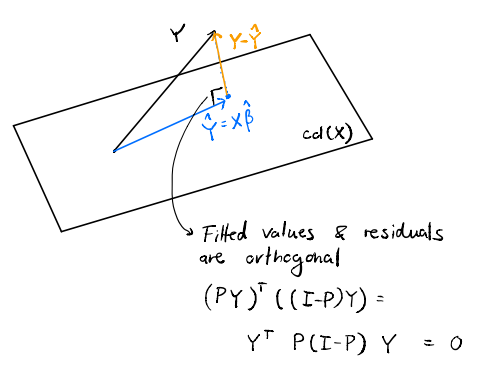
\includegraphics[height=5cm]{06-geometric} 
\end{figure}

\subsection{Normal linear model}

The normal linear model is a linear model under the assumption that $\varepsilon \sim N(0,\sigma^2 I)$, where $\sigma^2$ is unknown.
The parameters in the model are now $(\beta, \sigma^2)$.
The likelihood function in the normal linear model is
\begin{align*}
	L(\beta, \sigma^2) = f_Y(y\mid \beta,\sigma^2) = (2\pi \sigma^2)^{-\frac{n}{2}} \exp{-\frac{1}{2\sigma^2} \sum_i (Y_i - x_i^\tran \beta)^2}
\end{align*}
The log-likelihood is
\begin{align*}
	\ell(\beta,\sigma^2) = \text{constant} - \frac{n}{2}\log \sigma^2 - \frac{1}{2\sigma^2} \norm{Y-X\beta}^2
\end{align*}
To maximise this as a function of $\beta$ for any fixed $\sigma^2$, we must minimise the residual sum of squares $S(\beta) = \norm{Y-X\beta}^2$.
So $\hat \beta = (X^\tran X)^{-1} X^\tran Y$ is the maximum likelihood estimator of $\beta$.
Further, $\hat \sigma^2 = n^{-1} \norm{Y-X\hat\beta}^2 = n^{-1} \norm{\hat Y - Y}^2 = n^{-1} \norm{(I-P)Y}^2$.

\begin{theorem}
	In the normal linear model,
	\begin{enumerate}
		\item $\hat \beta \sim N(\beta,\sigma^2(X^\tran X)^{-1})$;
		\item $n\frac{\hat\sigma^2}{\sigma^2} \sim \chi^2_{n-p}$;
		\item $\hat \beta, \hat \sigma^2$ are independent.
	\end{enumerate}
\end{theorem}

\begin{proof}
	We prove each part separately.
	\begin{enumerate}
		\item We already know that $\expect{\hat \beta} = \beta$, and $\Var{\hat \beta} = \sigma^2 (X^\tran X)^{-1}$.
		      So it suffices to show that $\hat \beta$ is a MVN.
		      Since $\hat \beta = (X^\tran X)^{-1} X^\tran Y$, it is a linear function of $Y$ which is a MVN, so $\hat \beta$ is a MVN.
		\item Observe that
		      \begin{align*}
			      n\frac{\hat\sigma^2}{\sigma^2} = \frac{\norm{(I-P)Y}^2}{\sigma^2} = \frac{\norm{(I-P)(X\beta+\varepsilon)}^2}{\sigma^2}
		      \end{align*}
		      Since $(I-P)X = 0$ as $P$ is the orthogonal projection onto the column space of $X$,
		      \begin{align*}
			      n\frac{\hat\sigma^2}{\sigma^2} = \frac{\norm{(I-P)\varepsilon}^2}{\sigma^2} \sim \chi^2_{\tr (I-P)}\footnote{By \Cref{thm:6.1}}
		      \end{align*}
		      where $\tr (I-P) = \tr I - \tr P = n - p$ since $X \in \mathbb R^{n \times p}$ is assumed to have full rank.
		\item Note that $\hat \sigma^2$ is a function of $(I-P)\varepsilon$, and
		      \begin{align*}
			      \hat\beta &= (X^\tran X)^{-1} X^\tran Y \\
			                &= (X^\tran X)^{-1} X^\tran (X\beta+\varepsilon) \\
			                &= \beta + (X^\tran X)^{-1} X^\tran \varepsilon \\
			                &= \beta + (X^\tran X)^{-1} X^\tran P\varepsilon\footnote{$X^\tran P = X^\tran$ as $P$ acts as the identity in the column space of $X$.}
		      \end{align*}
		      is a function of $P\varepsilon$.
		      Since $(I-P)\varepsilon$ and $P \varepsilon$ are independent by \Cref{thm:6.1}, so are $\hat \beta, \hat \sigma^2$.
	\end{enumerate}
\end{proof}

\begin{corollary}
	$\hat{\sigma}^2$ is biased, but asymptotically unbiased.
\end{corollary} 

\begin{proof}
	\begin{align*}
		\expect{\frac{n\hat\sigma^2}{\sigma^2}} = \expect{\chi^2_{n-p}} = n-p \implies \expect{\hat\sigma^2} = \sigma^2 \cdot \frac{n-p}{n} < \sigma^2
	\end{align*}
\end{proof} 

\subsection{Inference}

\begin{definition}[$t$-distribution]
	Let $U \sim N(0,1)$ and $V \sim \chi^2_n$ be independent random variables.
	Then
	\begin{align*}
		T = \frac{U}{\sqrt{\frac{V}{n}}}
	\end{align*}
	has a \vocab{$t_n$-distribution}.
\end{definition}

As $n \to \infty$, this approaches the standard normal distribution.

\begin{definition}[$F$-distribution]
	Let $V \sim \chi^2_n$ and $W \sim \chi^2_m$ be independent random variables.
	Then
	\begin{align*}
		F = \frac{V/n}{W/m}
	\end{align*}
	has an \vocab{$F_{n,m}$-distribution}.
\end{definition}

\begin{example}
	We consider a $100(1-\alpha)\%$ confidence interval for one of the coefficients $\beta$ in the normal linear model $Y = X\beta + \varepsilon$.
	Without loss of generality, we will consider $\beta_1$.

	We begin by finding a \textit{pivot}, which is a distribution that does not depend on the parameters of the model.
	By standardising the above form of $\hat \beta$,
	\begin{align*}
		\frac{\beta_1 - \hat \beta_1}{\sqrt{\sigma^2(X^\tran X)^{-1}_{11}}} \sim N(0,1)
	\end{align*}
	where $M^{-1}_{11}$ is the top left entry in the matrix $M^{-1}$.
	This random variable is independent from $\frac{n\hat \sigma^2}{\sigma^2} \sim \chi^2_{n-p}$.
	Now, to construct a pivot, we find
	\begin{align*}
		\frac{\frac{\beta_1 - \hat \beta_1}{\sqrt{\sigma^2(X^\tran X)^{-1}_{11}}}}{\sqrt{\frac{\hat \sigma^2}{\sigma^2} \cdot \frac{n}{n-p}}} \sim \frac{U}{\sqrt{\frac{V}{n}}} \sim t_{n-p}
	\end{align*}
	The $\sigma^2$ terms cancel, so the statistic is a function only of $\beta_1$ and functions of the data.
	Then,
	\begin{align*}
		\psub{\beta,\sigma^2}{ -t_{n-p}\qty(\frac{\alpha}{2}) \leq \frac{\hat \beta_1 - \beta_1}{\sqrt{(X^\tran X)^{-1}_{11}}} \sqrt{\frac{n-p}{n\hat\sigma^2}} \leq t_{n-p}\qty(\frac{\alpha}{2}) } = 1-\alpha
	\end{align*}
	since the $t$ distribution is symmetric about zero.
	Rearranging to find an interval for $\beta_1$,
	\begin{align*}
		\psub{\beta,\sigma^2}{
			\hat \beta_1 - t_{n-p}\qty(\frac{\alpha}{2}) \frac{\sqrt{(X^\tran X)^{-1}_{11} \hat\sigma^2}}{\sqrt{(n-p)/n}}
			\leq \beta_1 \leq
			\hat \beta_1 + t_{n-p}\qty(\frac{\alpha}{2}) \frac{\sqrt{(X^\tran X)^{-1}_{11} \hat\sigma^2}}{\sqrt{(n-p)/n}}
		} = 1-\alpha
	\end{align*}
	Hence,
	\begin{align*}
		I = \qty[\hat \beta_1 \pm t_{n-p}\qty(\frac{\alpha}{2}) \frac{\sqrt{(X^\tran X)^{-1}_{11} \hat \sigma^2}}{\sqrt{(n-p)/n}} ]
	\end{align*}
	is a $100(1-\alpha)\%$ confidence interval for $\beta_1$.

	Consider a test for $H_0 \colon \beta_1 = \beta^\star$, $H_1 \colon \beta_1 \neq \beta^\star$.
	By connecting tests and confidence intervals, we can test $H_0$ with size $\alpha$ by rejecting this null hypothesis when $\beta^\star$ is not contained within the confidence interval $I$ for $\beta_1$.

	Consider a special case where $Y_1, \dots, Y_n \overset{\text{iid}}{\sim} N(\mu,\sigma^2)$ where $\mu, \sigma^2$ are unknown, and we want to infer results about $\mu$.
	Note that this is a special case of the normal linear model where
	\begin{align*}
		X = \begin{pmatrix}
			1      \\
			\vdots \\
			1
		\end{pmatrix};\quad \beta = \begin{pmatrix}
			\mu
		\end{pmatrix}
	\end{align*}
	So we can infer a confidence interval for $\mu$ using the above statistic.
\end{example}

\begin{example}
	Consider a $100(1-\alpha)\%$ confidence set for $\beta$ as a whole.
	Note that
	\begin{align*}
		\hat \beta - \beta \sim N(0,\sigma^2 (X^\tran X)^{-1})
	\end{align*}
	As $X$ has full rank, $X^\tran X$ is positive definite.
	So it has eigendecomposition $X^\tran X = U D U^\tran$ where $D_{ii} > 0$ and $D$ diagonal.
	We define
	\begin{align*}
		(X^\tran X)^\alpha = U D^\alpha U^\tran
	\end{align*} 
	Then,
	\begin{align*}
		(X^\tran X)^{1/2} (\hat \beta - \beta) \sim N(0,\sigma^2(X^\tran X)^{1/2} (X^\tran X)^{-1} (X^\tran X)^{1/2}) \sim N(0,\sigma^2 I).
	\end{align*}
	Hence,
	\begin{align*}
		\frac{\norm{(X^\tran X)^{1/2} (\hat \beta - \beta)}^2}{\sigma^2} \sim \chi^2_p
	\end{align*} as this is the sum of $p$ standard normals.
	We can also write this as
	\begin{align*}
		\frac{\norm{(X^\tran X)^{1/2} (\hat \beta - \beta)}^2}{\sigma^2} = \frac{\norm{X(\hat \beta - \beta)}^2}{\sigma^2}
	\end{align*}
	Since this is a function of $\hat \beta$, this is independent of any function of $\hat \sigma^2$.
	In particular, it is independent of $\frac{n\hat\sigma^2}{\sigma^2} \sim \chi^2_{n-p}$.
	Thus, we can form a pivot by
	\begin{align*}
		\frac{\norm{X(\hat \beta - \beta)}^2 / (\sigma^2 p)}{\hat\sigma^2 n / (\sigma^2(n-p))} \sim \frac{\chi^2_p / p}{\chi^2_{n-p} / (n-p)} \sim F_{p,n-p}
	\end{align*}
	This does not depend on $\sigma^2$.
	For all $\beta, \sigma^2$,
	\begin{align*}
		\psub{\beta,\sigma^2}{
			\frac{\norm{X(\hat \beta - \beta)}^2 / p}{\hat\sigma^2 n / (n-p)}
			\leq F_{p,n-p}(\alpha)} = 1-\alpha
	\end{align*}
	because the $F$ distribution has support only on the positive real line.
	It is nontrivial to express this as a region for $\beta$ since it is vector-valued.
	We can say, however, that
	\begin{align*}
		\qty{\beta' \in \mathbb R^p \colon \frac{\norm{X(\hat \beta - \beta)}^2/p}{\hat \sigma^2 n/(n-p)} \leq F_{p,n-p}(\alpha)}
	\end{align*}
	is a $100(1-\alpha)\%$ confidence set for $\beta$.

	This set is an ellipsoid centred at $\hat \beta$.
	The shape of the ellipsoid depends on the design matrix $X$; the principal axes are given by eigenvectors of $X^\tran X$.
\end{example}
The above two results are exact; no approximations were made.

\subsection{F-tests}
We wish to test whether a collection of predictors $\beta_i$ are equal to zero.
Without loss of generality, we will take the first $p_0 \leq p$ predictors.
We have $H_0 \colon \beta_1 = \dots = \beta_{p_0} = 0$, and $H_1 = \beta \in \mathbb R^p$.
We denote $X = (X_0, X_1)$ as a block matrix with $X_0 \in \mathbb R^{n \times p_0}$ and $X_1 \in \mathbb R^{n \times (p-p_0)}$, and we denote $\beta = (\beta^0, \beta^1)^\tran$ similarly.
The null model has $\beta^0 = 0$.
This is a linear model $Y = X\beta + \varepsilon = X_1 \beta^1 + \varepsilon$.
We will write $P = X(X^\tran X)^{-1} X^\tran$ and $P_1 = X_1 (X_1^\tran X_1)^{-1} X_1^\tran$.
Note that as $X$ and $P$ have full rank, so must $X_1, P_1$.

\begin{lemma}
	$(I-P)(P - P_1) = 0$, and $P - P_1$ is an orthogonal projection with rank $p_0$.
\end{lemma}

\begin{proof}
	$P - P_1$ is symmetric since $P$ and $P_1$ are symmetric.
	It is also idempotent, since
	\begin{align*}
		(P-P_1)(P-P_1) = P^2 - P_1 P - P P_1 + P_1^2 = P - P_1 - P_1 + P_1 = P - P_1
	\end{align*}
	since $P_1$ projects onto the column space of $X_1$ so $P_1 P = P_1$.
	Hence $P - P_1$ is indeed an orthogonal projection matrix.
	The rank is $\rank(P - P_1) = \tr(P - P_1) = \tr P - \tr P_1 = p - (p - p_0) = p_0$.
	Also,
	\begin{align*}
		(I-P)(P-P_1) = P-P_1 - P + PP_1 = P-P_1 - P + P_1 = 0
	\end{align*}
\end{proof}

Recall that the maximum log-likelihood in the normal linear model is given by
\begin{align*}
	\ell(\hat \beta, \hat \sigma^2) = \frac{-n}{2} \log \hat\sigma^2 - \frac{n}{2} \cdot \text{constant} = \frac{-n}{2} \log \frac{\norm{(I-P)Y}^2}{n} + \text{constant}
\end{align*}

The generalised likelihood ratio statistic is
\begin{align*}
	2 \log \Lambda &= 2\qty( \sup_{\beta \in \mathbb R^p,\sigma^2>0} \ell(\beta, \sigma^2) -  \sup_{\beta_0 = 0, \beta_1 \in \mathbb R^{p-p_0},\sigma^2>0} \ell(\beta, \sigma^2) )\\
	&= n \qty[ -\log \frac{\norm{(I-P)Y}^2}{n} + \log \frac{\norm{(I-P_1)Y}^2}{n} ]
\end{align*}

Wilks' theorem applies here, showing that $2 \log \Lambda \sim \chi^2_{p_0}$ asymptotically as $n \to \infty$ with $p, p_0$ fixed.
However, we can find an exact test, so using Wilks' theorem will not be necessary.
$2 \log \Lambda$ is monotone in

\begin{align*}
	\frac{\norm{(I-P_1)Y}^2}{\norm{(I-P)Y}^2} & = \frac{\norm{(I-P+P-P_1)Y}^2}{\norm{(I-P)Y}^2} \\
	&= \frac{\norm{(I-P)Y}^2 + \norm{(P-P_1)Y}^2 + 2Y^\tran (I-P)(P-P_1) Y}{\norm{(I-P)Y}^2} \\
	&= \frac{\norm{(I-P)Y}^2 + \norm{(P-P_1)Y}^2}{\norm{(I-P)Y}^2} \\
	&= 1 + \frac{\norm{(P-P_1)Y}^2}{\norm{(I-P)Y}^2}
\end{align*}

The generalised likelihood ratio test rejects when the $F$-statistic
\begin{align*}
	F = \frac{\norm{(P-P_1)Y}^2}{\norm{(I-P)Y}^2} \cdot \frac{1/p_0}{1/(n-p)}
\end{align*}
is large.

\begin{theorem}
	Under $H_0\colon \beta_1 = \dots = \beta_{p_0} = 0$, in the normal linear model,
	\begin{align*}
		F = \frac{\norm{(P-P_1)Y}^2}{\norm{(I-P)Y}^2} \cdot \frac{1/p_0}{1/(n-p)} \sim F_{p_0,n-p}
	\end{align*}
\end{theorem}

\begin{proof}
	Recall that
	\begin{align*}
		\norm{(I-P)Y}^2 = \norm{(I-P)\varepsilon}^2 \sim \chi^2_{n-p} \cdot \sigma^2
	\end{align*}
	Therefore it suffices to show that $\norm{(P-P_1)Y}^2$ is an independent $\chi^2_{p_0} \cdot \sigma^2$ random variable.
	Under $H_0$, we have that
	\begin{align*}
		(P-P_1)Y = (P-P_1)(X\beta+\varepsilon) = (P-P_1)(X_1 \beta^1 + \varepsilon) = (P-P_1)\varepsilon
	\end{align*}
	since $P, P_1$ preserve $X_1$.
	Hence, $\norm{(P-P_1)Y}^2 = \norm{(P-P_1)\varepsilon}^2 \sim \chi^2_{\rank (P-P_1)} \cdot \sigma^2 = \chi^2_{p_0} \cdot \sigma^2$.

	We must now show independence between $(I-P)Y$ and $(P-P_1)Y$.
	The vectors $(I-P)\varepsilon, (P-P_1)\varepsilon$ are independent; indeed,
	\begin{align*}
		E = \begin{pmatrix}
			(I-P)\varepsilon \\
			(P-P_1)\varepsilon
		\end{pmatrix}
	\end{align*}
	is a multivariate normal vector, and
	\begin{align*}
		\expect{E} = 0;\quad \Var E = \begin{pmatrix}
			I-P          & (I-P)(P-P_1) \\
			(I-P)(P-P_1) & P-P_1
		\end{pmatrix} = \begin{pmatrix}
			I-P & 0     \\
			0   & P-P_1
		\end{pmatrix}
	\end{align*}
	and since $(I-P)\varepsilon$ and $(P-P_1)\varepsilon$ are elements of a multivariate normal vector and are uncorrelated, they are independent as required.
\end{proof}

The generalised likelihood ratio test of size $\alpha$ rejects $H_0$ when $F > F^{-1}_{p_0,n-p}(\alpha)$.
This is an exact test for all $n, p, p_0$.
Previously, we found a test for $H_0\colon \beta_1 = 0$ against $H_1 \colon \beta_1 \neq 0$.
This is a special case of the $F$-test derived above, where $p_0 = 1$.
The previous test of size $\alpha$ rejects $H_0$ when
\begin{align*}
	\abs{\hat\beta} > t_{n-p}\qty(\frac{\alpha}{2}) \sqrt{\frac{\hat\sigma^2 n (X^\tran X)^{-1}_{11}}{n-p}}
\end{align*}

\begin{lemma}
	This test is equivalent to the $F$-test with $p_0 = 1$.
\end{lemma} 

This proof was left as an exercise to the reader.

\begin{proof}
	We will show that these two tests are equivalent; they reject $H_0$ in the same critical region.
	The $t$-test rejects if and only if
	\begin{align*}
		\hat \beta_1^2 > t_{n-p}\qty(\frac{\alpha}{2})^2 \frac{\hat\sigma^2 n (X^\tran X)^{-1}_{11}}{n-p}
	\end{align*}
	Note that $t_{n-p}\qty(\frac{\alpha}{2})^2 = F_{1,n-p}(\alpha)$, since
	\begin{align*}
		U \sim N(0,1);\;W \sin \chi^2_n \implies T = \frac{U}{\sqrt{W/n}} \implies T^2 = \frac{U^2}{W/n} = \frac{V/1}{W/n} \sim F_{1,n}
	\end{align*}
	where $V \sim \chi^2_1$.
	Hence,
	\begin{align*}
		\frac{\hat \beta_1/(X^\tran X)^{-1}_{11}}{\hat\sigma^2 n/(n-p)} > F_{1,n-p}(\alpha)
	\end{align*}
	It suffices to show that
	\begin{align*}
		\frac{\hat \beta_1}{(X^\tran X)^{-1}_{11}} = \frac{\norm{(P-P_1)Y}^2}{\underbrace{p_0}_{=1}};\quad \frac{\hat \sigma^2 n}{n-p} = \frac{\norm{(I-P)Y}^2}{n-p}
	\end{align*}
	We have already shown the latter part.
	For $\hat \beta_1$, note that in this case, $P - P_1$ is a projection of rank 1 onto the one-dimensional subspace spanned by the vector $v = (I-P)X^0$ where $X^0$ is the first column in the matrix $X$.
	First, note the following identity.
	\begin{align*}
		X_0^\tran (I - P_1) = v^\tran = v^\tran (P-P_1) = X_0^\tran (I-P_1)(P-P_1) = X_0^\tran (I-P_1)P
	\end{align*}
	Then,
	\begin{align*}
		\norm{(P-P_1)Y}^2 &= \norm{\frac{v}{\norm{v}} \qty(\frac{v}{\norm{v}})^\tran Y}^2 \\
		&= \frac{(v^\tran Y)^2}{\norm{v}^2} = \frac{(X_0^\tran (I-P_1) Y)^2}{\norm{(I-P_1) X_0}^2} \\
		&= \frac{(X_0^\tran (I-P_1) P Y)^2}{\norm{(I-P_1) X_0}^2} \\
		&= \frac{(X_0^\tran (I-P_1) X \hat\beta)^2}{\norm{(I-P_1) X_0}^2}
	\end{align*}
	Note that $(I-P_1) X = [(I-P_1)X_0, 0, \dots, 0]$.
	Hence,
	\begin{align*}
		\norm{(P-P_1)Y}^2 &= \frac{\norm{(I-P_1)X_0}^4 \hat \beta_1}{\norm{(I-P_1)X_0}^2} \\
		&= \norm{(I-P_1)X_0}^2 \hat \beta_1
	\end{align*}
	Finally, we show that
	\begin{align*}
		(X^\tran X)^{-1}_{11} = \frac{1}{\norm{(I-P_1)X_0}^2}
	\end{align*}
	using the Woodbury identity for blockwise matrix inversion.
	Hence,
	\begin{align*}
		\frac{\hat\beta_1^2}{(X^\tran X)^{-1}_{11}} = \norm{(P-P_1) Y}^2
	\end{align*}
	as required.
\end{proof}

\subsection{Analysis of variance}
Suppose we have categorical predictors.

\begin{example}
	Let $Y_i \in \mathbb{R}$ be the clinical response.
	$z_i \in \{\text{control}, \text{treatment 1}, \text{treatment 2}\}$, this is categorical.
	Let $x_{ij} = 1_{z_i = j}$, i.e. is subject $i$ was in group $j$.
	$x_i \in \mathbb{R}^3$ so it is numerical.

	Say our model is $Y_i = \alpha + \beta_1 x_{i, 1} + \beta_2 x_{i,2} + \beta_3 x_{i, 3}$\footnote{I think $Y_{ij} = \alpha + \beta_j x_{ij} + \epsilon_{ij}$ where $\epsilon_{ij} \sim \mathcal{N}(0, \sigma^2)$ independent.}.
	In this case, \begin{align*}
		X = \begin{pmatrix}
			1      & 1 		& 0      & 0      \\
			1      & 1 		& 0      & 0      \\
			\vdots & \vdots & \vdots & \vdots \\
			1      & 0 		& 1      & 0      \\
			1      & 0 		& 1      & 0      \\
			\vdots & \vdots & \vdots & \vdots \\
			1      & 0 		& 0      & 1      \\
			1      & 0 		& 0      & 1
		\end{pmatrix}.
	\end{align*} 
	This has rank $3 < 4$ so to deal with this we add a corner point constraint.
	This is where we call one of the groups the ``baseline'' and remove it from the linear model.
	In this case we set $\beta_1 = 0$, removing the second column from $X$.

	The interpretation of $\beta_j$ depends on the baseline, $\beta_j$ is the the effect of being in group $j$ relative to the baseline.

	However $\operatorname{col}(X)$ and the matrix $P$ are insensitive to the choice of baseline.
	Therefore so are the fitted values, $\hat{Y} = PY$.

	This can be extended to a model with more than $1$ categorical predictor e.g. treatment group and gender. 
\end{example} 

% Suppose we investigate responses of patients after receiving one of three treatments, including a control, which will be given index 1.
% We will consider only one predictor, denoting which treatment a given patient received.
% Consider the linear model
% \begin{align*}
% 	Y_{ij} = \alpha + \mu_j + \varepsilon_{ij}
% \end{align*}
% where $j = 1, 2, 3$ is the treatment index, and $i = 1, \dots, N$ is the index of a patient in a given group.
% Let $(\varepsilon_{ij}) \sim N(0, \sigma^2)$ be independent.
% Without loss of generality, we can set $\mu_1 = 0$, since we have an additional parameter $\alpha$; this is known as a \textit{corner point} constraint.
% Then, $\mu_j$ should be interpreted as the effect of treatment $j$ relative to treatment 1, which in this case is the control.

\begin{definition}[Analysis of Variance (ANOVA)]
	The \vocab{analysis of variance (ANOVA)} test on the linear model
	\begin{align*}
		Y_{ij} = \alpha + \beta_j x_{ij} + \varepsilon_{ij}
	\end{align*}
	where $\beta_1 = 0$ is given by
	\begin{align*}
		H_0 \colon \beta_2 = \beta_3 = \dots = 0, \alpha \neq 0;\quad H_1 \colon \beta_2, \beta_3, \dots, \alpha \in \mathbb R
	\end{align*}
	In particular, $H_0$ gives $\expect{Y_{ij}} = \alpha$.
\end{definition}

In our example, $H_0 \colon \beta_2 = \beta_3 = 0, \alpha \neq 0$ and $H_1 \colon \beta_2, \beta_3, \alpha \in \mathbb R$.
This is a special case of the $F$-test, since we are testing whether the coefficients $\beta_i$ are equal to zero.
\begin{align*}
	X = \begin{pmatrix}
		1      & 0      & 0      \\
		1      & 0      & 0      \\
		\vdots & \vdots & \vdots \\
		1      & 1      & 0      \\
		1      & 1      & 0      \\
		\vdots & \vdots & \vdots \\
		1      & 0      & 1      \\
		1      & 0      & 1
	\end{pmatrix} = \begin{pmatrix}
		X_1 & X_0
	\end{pmatrix}
\end{align*}
The first column of $X$, denoted $X_1$, represents $\alpha$, and the other columns, denoted $X_0$, represent $\mu_2, \mu_3$.
$X_0$ is eliminated under the null hypothesis.

Note that $X$ has $3N$ rows, where each block of $N$ consecutive rows is identical.
Recall that the $F$-test uses the test statistic

\begin{align*}
	F = \frac{\norm{(P-P_1)Y}^2}{\norm{(I-P)Y}^2} \cdot \frac{1/p_0}{1/(n-p)} \sim F_{p_0,n-p}
\end{align*}

For this test, $P$ projects onto the space of vectors in $\mathbb R^{3N}$ which are constant over treatment groups.
In other words, let
\begin{align*}
	\overline Y_j = \frac{1}{N} \sum_{i=1}^N Y_{ij}
\end{align*}

Then,
\begin{align*}
	P Y = \qty( \underbrace{\overline Y_1, \dots, \overline Y_1}_{N \text{ entries}}, \underbrace{\overline Y_2, \dots, \overline Y_2}_{N \text{ entries}}, \underbrace{\overline Y_3, \dots, \overline Y_3}_{N \text{ entries}} )^\tran
\end{align*}
$P_1$ projects onto the subspace of constant vectors in $\mathbb R^{3N}$, i.e. $P_1 = \frac{1}{N} 1 1^\tran$ so
\begin{align*}
	\overline Y = \frac{1}{3N} \sum_{i=1}^N \sum_{j=1}^3 Y_{ij} \implies P_1 Y = \qty( \underbrace{\overline Y, \dots, \overline Y}_{3N \text{ entries}} )^\tran
\end{align*}

Hence, we can write the $F$ statistic as
\begin{align*}
	F = \frac{\sum_{j=1}^3 N \qty(\overline Y_j - \overline Y)^2 / 2}{\sum_{i=1}^N \sum_{j=1}^3 \qty(Y_{ij} - \overline Y_j)^2 / (3N-3)}
\end{align*}

We can generalise this to the case where there are $J > 3$ treatment groups:
\begin{align*}
	F = \frac{\sum_{j=1}^J N \qty(\overline Y_j - \overline Y)^2 / (J-1)}{\sum_{i=1}^N \sum_{j=1}^J \qty(Y_{ij} - \overline Y_j)^2 / (JN-J)} = \frac{\text{variance between treatments}}{\text{variance within treatments}}
\end{align*}

\begin{remark}
	This test is sometimes called \textit{one-way} analysis of variance.
	\textit{Two-way} analysis of variance is a similar analysis in an experiment where groups are defined according to two variables.
	For instance, the response could be a student's performance in an exam, where the treatments are
	\begin{enumerate}
		\item completion of supervisions (zero representing not complete, one representing complete); and
		\item whether a monetary incentive was given (zero representing no incentive, one representing an incentive).
	\end{enumerate}
	Here, we would have the result $Y_{ijk}$ as the number of marks of student $i$ in group $(j,k)$.
	The model would be
	\begin{align*}
		Y_{ijk} = \alpha + \mu_j + \lambda_k + \varepsilon_{ijk}
	\end{align*}
	with a constraint without loss of generality that $\mu_0 = \lambda_0 = 0$.
	The two-way analysis of variance test is then
	\begin{align*}
		H_0 \colon \mu_1 = \lambda_1 = 0;\quad H_1 \colon \mu_1, \lambda_1 \in \mathbb R
	\end{align*}
\end{remark}

\subsection{Simple linear regression - Non Examinable}
In a linear regression model, we often centre predictors to simplify certain expressions.
\begin{align*}
	Y_i = \alpha + \beta (x - \overline x) + \varepsilon_i
\end{align*}
where $\overline x = \frac{1}{n} \sum_{i=1}^n x_i$, and the $\varepsilon_i$ independently have the usual $N(0, \sigma^2)$ distribution.
In this case, the maximum likelihood estimator $(\hat \alpha, \hat \beta)$ takes a simple form.
Recall that $(\hat \alpha, \hat \beta)$ minimises
\begin{align*}
	S(\alpha, \beta) = \sum_{i=1}^n \qty(Y_i - \alpha - \beta(x_i - \overline x))^2
\end{align*}
Hence,
\begin{align*}
	\pdv{S(\alpha, \beta)}{\alpha} = \sum_{i=1}^n -2\qty(Y_i - \alpha - \beta(x_i - \overline x)) = \sum_{i=1}^n -2\qty(Y_i - \alpha)
\end{align*}
This gives the simple expression
\begin{align*}
	\alpha = \frac{\sum_{i=1}^n Y_i}{n} = \overline Y
\end{align*}
Now,
\begin{align*}
	\eval{\pdv{S(\alpha, \beta)}{\beta}}_{\alpha = \hat \alpha} = \sum_{i=1}^n -2\qty(Y_i - \overline Y - \beta(x_i - \overline x))(x_i - \overline x)
\end{align*}
This vanishes when
\begin{align*}
	\hat \beta = \frac{\sum_{i=1}^n \qty(Y_i - \overline Y)(x_i - \overline x)}{\sum_{i=1}^n (x_i - \overline x)^2} = \frac{S_{xy}}{S_{xx}}
\end{align*}
Note that $\frac{S_{xy}}{n}$ is the sample covariance of $X$ and $Y$, and $\frac{S_{xx}}{n}$ is the sample variance of $X$.

\end{document}